\section{Multivariate discriminant}
\label{sec:tmva}


%%%%%%%%%%%%%%%
\begin{table*}[t!]
  \caption{\small{Discriminating variables (n) used in the training of the BDT of each SR. 
The ranking of the input variables according to their importance in the training is reported from highest (1) to 
lowest (n). Variables whose ranking is missing are not included in the training of the corresponding SR. The description of each variable is provided in the text.}}
%Variables are ranked from highest (1) to lowest (n) relative to one another by their
%      importance in the training. Variables which do not have a ranking are not included in the training. 
%The values represent their ra importance rankings of each variable and cross($\times$) denotes the variable is not used in the training.
%      The descriptions of each variable are provided in the following text.}}
\label{tab:importance}
 \centering
 \begin{tabular}{cccccccc} \toprule\toprule
   & $t_{l}\tauhad$-1j                                  &  $t_{h}\tlhad$-2j   &  $t_{l}\tauhad$-2j & $t_{h}\tlhad$-3j & $t_{\ell}2\tauhad$     & $t_h2\tauhad$-2j & $t_h2\tauhad$-3j       \\\midrule
   Total variables~(n)                           & $12$ & $15$ & $12$ & $17$ & $15$ & $12$ & $12$ \\\midrule 
 $m_{\text{jj}}$                                      &   &             &           & $9$      &       & $6$      & $7$\\
 $\chi^{2}$                                          &   &             &           & $14$     &       &  &       \\
 \text{max}($\eta_{\tau}$)                           & $4$       &             &  $4$              &  & $10$          &  &        \\
 $m^{W}_{\text{T}}$                           & $11$      &             &  $8$              &  & $13$          &  &         \\
 $m_{\tau\tau,\text{fit}}$                                     &   &  $2$                &           & $3$      &       & $1$      & $1$          \\
 $m_{\text{bjj},\text{fit}}$                            &   &  $1$                &           & $2$      &       & $3$      & $4$          \\
 ${\pt}^{\ell}$                                 & $12$      &  $15$               &  $12$             & $17$     &       &  &         \\
 $m_{\tau\tau\text{q},\text{fit}}$                          &   &             &           &  &       & $10$     & $6$\\
 $m_{\text{bjj}}$                 & $3$       &             &  $5$              &  & $4$           &  &         \\
 ${\pt}_{\tau1}$                                 & $1$       &  $4$                &  $1$              & $1$      & $5$           & $11$   & $10$           \\
 $\met$                                              & $5$       &  $11$               &  $10$             & $13$     & $6$           & $7$    & $13$          \\
 $m_{\tau\tau}$                           & $10$      &  $14$               &  $11$             & $6$      & $1$           & $2$    & $2$          \\
 $E_{\tau1}/E_{\tau1,\text{fit}}$                  &   &  $10$               &           & $12$     &       & $8$    & $8$          \\
 $E_{\tau2}/E_{\tau2,\text{fit}}$                  &   &  $7$                &           & $4$      &       & $9$    & $11$         \\
 ${\pt}_{\tautau} $                          &   &             &           &  & $9$           &  &         \\
 $m_{\tau\tau\text{q}}$               &   &             &           &  & $3$           &  &        \\
 $\Delta\phi(\tau\tau,\met)$                         &   &  $6$                            &           & $16$     &       & $13$   & $12$         \\
 $\met\text{centrality}$                             &   &  $13$               &           & $15$     &       & $12$   & $9$         \\
 \text{min}($m_{\tau\tau \text{j}}$)             & $9$       &             &  $3$              &  & $14$          &  &         \\
 \text{min}($\Delta R(\ell,\tau)$)                               & $8$       &  $9$                &  $9$              & $10$     & $15$          &  &         \\
 $\Delta R(\tau,\tau)$                               &   &             &           &  & $2$           & $4$    & $3$             \\
 $\Delta R(\ell,\text{$b$-jet})$                       & $2$       &  $3$                &  $2$              & $8$      & $12$          &  &         \\
 $\Delta R(\tau1,\text{$b$-jet})$                       & $6$       &  $5$                &  $6$              & $7$      & $11$          &  &        \\
 $\Delta R(\ell+\text{$b$-jet},\tau\tau )$             &   &             &           &  & $7$           &  &         \\
 $\Delta R(\tau1,\text{light-jet})$                   & $7$       &  $8$                &  $7$              & $5$      & $8$           & $5$    & $5$    \\
 \text{min}($m_{jj}$) &   &  $12$               &           & $11$     &       &  &         \\
% $m_{\text{W}}$                                      & $\times$  &  $\times$           &  $\times$         & $9$      & $\times$      & $6$      & $7$\\
% $\chi^{2}$                                          & $\times$  &  $\times$           &  $\times$         & $14$     & $\times$      & $\times$ & $\times$      \\
% \text{max}($\eta_{\tau}$)                           & $4$       &  $\times$           &  $4$              & $\times$ & $10$          & $\times$ & $\times$       \\
% $m^{\text{T}}_{\text{W}}$                           & $10$      &  $\times$           &  $8$              & $\times$ & $13$          & $\times$ & $\times$        \\
% $m_{\tau,\tau}$                                     & $\times$  &  $2$                &  $\times$         & $3$      & $\times$      & $1$      & $1$          \\
% $m_{\text{t},\text{SM}}$                            & $\times$  &  $1$                &  $\times$         & $2$      & $\times$      & $3$      & $4$          \\
% $p_{\text{T},\ell}$                                 & $12$      &  $15$               &  $12$             & $17$     & $\times$      & $\times$ & $\times$        \\
% $m_{\text{t},\text{FCNC}}$                          &  $\times$ &  $\times$           &  $\times$         & $\times$ & $\times$      & $10$     & $6$\\
% $m_{\text{t},\text{SM},\text{vis}}$                 & $3$       &  $\times$           &  $5$              & $\times$ & $4$           & $\times$ & $\times$        \\
% $p_{\text{T},\tau}$                                 & $1$       &  $4$                &  $1$              & $1$      & $5$           & $11$   & $10$           \\
% $\met$                                              & $5$       &  $11$               &  $10$             & $13$     & $6$           & $7$    & $13$          \\
% $m_{\tau\tau,\text{vis}}$                           & $10$      &  $14$               &  $11$             & $6$      & $1$           & $2$    & $2$          \\
% $E_{\text{vis}~\tau,1}/E_{\tau,1}$                  & $\times$  &  $10$               &  $\times$         & $12$     & $\times$      & $8$    & $8$          \\
% $E_{\text{vis}~\tau,2}/E_{\tau,2}$                  & $\times$  &  $7$                &  $\times$         & $4$      & $\times$      & $9$    & $11$         \\
% $P_{\text{T,\tauhadvis}} $                          & $\times$  &  $\times$           &  $\times$         & $\times$ & $9$           & $\times$ & $\times$        \\
% $m_{\text{t},\text{FCNC},\text{vis}}$               & $\times$  &  $\times$           &  $\times$         & $\times$ & $3$           & $\times$ & $\times$       \\
% $\Delta\phi(\tau\tau,\met)$                         & $\times$  &  $6$    			   &  $\times$         & $16$     & $\times$      & $13$   & $12$         \\
% $\met\text{centrality}$                             & $\times$  &  $13$               &  $\times$         & $15$     & $\times$      & $12$   & $9$         \\
% \text{Min}($m_{\tau\tau \text{q-jet}}$)             & $9$       &  $\times$           &  $3$              & $\times$ & $14$          & $\times$ & $\times$        \\
% $\Delta R(\ell,\tau)$                               & $8$       &  $9$                &  $9$              & $10$     & $15$          & $\times$ & $\times$        \\
% $\Delta R(\tau,\tau)$                               & $\times$  &  $\times$           &  $\times$         & $\times$ & $2$           & $4$    & $3$             \\
% $\Delta R(\ell,\text{b-jet})$                       & $2$       &  $3$                &  $2$              & $8$      & $12$          & $\times$ & $\times$        \\
% $\Delta R(\tau,\text{b-jet})$                       & $6$       &  $5$                &  $6$              & $7$      & $11$          & $\times$ & $\times$       \\
% $\Delta R(\ell+\text{b-jet},\tau\tau )$             & $\times$  &  $\times$           &  $\times$         & $\times$ & $7$           & $\times$ & $\times$        \\
% $\Delta R(\tau,\text{light-jet})$                   & $7$       &  $8$                &  $7$              & $5$      & $8$           & $5$    & $5$    \\
% \text{Min}($m_{\text{light-jet},\text{light-jet}}$) & $\times$  &  $12$               &  $\times$         & $11$     & $\times$      & $\times$ & $\times$        \\
 \bottomrule\bottomrule\\
 \end{tabular}
\end{table*}




%%%%%%%%%%%%%%%
%%%  \begin{table*}[t!]
%%%    \caption{\small{Discriminating variables used in the training of the BDT for hadronic channel.
%%%        The values in percent (\%) represent the separation and importance of each variable.
%%%      The descriptions of each variable are provided in the following text.}}
%%%  \label{tab:importance_xTFW}
%%%  \centering
\begin{tabular}{ccc} \toprule\toprule
  & $t_h\thadhad$-2j & $t_h\thadhad$-3j\\\midrule
$m_{\text{W}}$                               & $7.62$ / $6.54$ & $7.00$ / $8.00$\\
$m_{\text{t},\text{SM}}$                            & $10.61$ / $10.55$ & $9.66$ / $9.64$\\
$p_{\text{T},\tau }$                         & $5.70$ / $6.96$ & $5.86$ / $5.13$\\
$\met$                        & $7.07$ / $5.76$ & $4.34$ / $5.77$\\
$m_{\tau\tau,\text{vis}}$                  & $10.72$ / $10.95$ & $11.26$ / $10.92$\\
$m_{\tau ,\tau }$                     & $14.36$ / $14.63$ & $14.77$ / $13.77$\\
$m_{\text{t},\text{FCNC}}$                          & $5.81$ / $7.01$ & $7.49$ / $8.24$\\
$\Delta R(\tau,\tau)$               & $10.27$ / $9.58$ & $10.00$ / $9.12$\\
$\Delta\phi(\tau\tau,\met)$ & $2.69$ / $5.71$ & $4.51$ / $5.03$\\
$\met \text{centrality}$             & $3.89$ / $4.68$ & $5.87$ / $5.51$\\
$E_{\text{vis}~\tau ,1}/E_{\tau ,1}$         & $6.56$ / $5.50$ & $6.32$ / $4.74$\\
$E_{\text{vis}~\tau ,2}/E_{\tau ,2}$         & $6.45$ / $5.21$ & $4.72$ / $7.37$\\
$\Delta R(\tau,\text{light-jet})$       & $8.26$ / $6.93$ & $8.20$ / $6.75$\\
\bottomrule\bottomrule\\
\end{tabular}

%%%  \end{table*}
%%%  
%%%  \begin{table*}[t!]
%%%    \caption{\small{Discriminating variables used in the training of the BDT for leptonic channel.
%%%        The values in percent (\%) represent the separation and importance of each variable.
%%%      The descriptions of each variable are provided in the following text.}}
%%%  \label{tab:importance_tthML}
%%%  \centering
\begin{tabular}{cccccc} \toprule\toprule
 & $t_{l}\tauhad$-1j & $t_{h}\tlhad$-2j & $t_{l}\tauhad$-2j & $t_{h}\tlhad$-3j & $t_l\thadhad$\\\midrule
 $m_{\text{W}}$ &  / &  / &  / & $5.96$ / $6.84$ &  /\\
$\chi^{2}$ &  / &  / &  / & $5.35$ / $5.08$ &  /\\
\text{max}($\eta_{\tau}$) & $8.98$ / $8.97$ &  / & $9.35$ / $10.04$ &  / & $6.27$ / $6.14$\\
$m^{\text{T}}_{\text{W}}$ & $6.97$ / $6.34$ &  / & $8.39$ / $8.15$ &  / & $4.78$ / $5.84$\\
$m_{\tau,\tau}$ &  / & $7.99$ / $7.85$ &  / & $7.28$ / $7.86$ &  /\\
$m_{\text{t},\text{SM}}$ &  / & $8.20$ / $8.13$ &  / & $7.54$ / $7.24$ &  /\\
$p_{\text{T},\ell}$ & $4.51$ / $5.17$ & $3.16$ / $3.93$ & $4.60$ / $5.62$ & $2.82$ / $3.52$ &  /\\
$m_{\text{t},\text{SM},\text{vis}}$ & $10.36$ / $10.05$ &  / & $9.15$ / $9.10$ &  / & $7.50$ / $7.06$\\
$p_{\text{T},\tau}$ & $12.28$ / $10.93$ & $7.52$ / $7.60$ & $11.63$ / $12.32$ & $7.68$ / $7.96$ & $7.28$ / $8.18$\\
$\met$ & $8.16$ / $6.83$ & $6.36$ / $6.28$ & $6.37$ / $5.72$ & $5.38$ / $4.47$ & $7.27$ / $6.11$\\
$m_{\tau\tau,\text{vis}}$ & $6.40$ / $6.95$ & $5.79$ / $6.65$ & $5.31$ / $4.89$ & $6.18$ / $6.00$ & $10.35$ / $10.09$\\
$E_{\text{vis}~\tau,1}/E_{\tau,1}$ &  / & $6.39$ / $5.90$ &  / & $5.35$ / $5.35$ &  /\\
$E_{\text{vis}~\tau,2}/E_{\tau,2}$ &  / & $6.94$ / $7.40$ &  / & $6.69$ / $6.54$ &  /\\
$P_{\text{T,\tauhadvis}} $ &  / &  / &  / &  / & $6.49$ / $6.36$\\
$m_{\text{t},\text{FCNC},\text{vis}}$ &  / &  / &  / &  / & $8.01$ / $7.43$\\
$\Delta\phi(\tau\tau,\met)$ &  / & $7.02$ / $6.96$ &  / & $4.97$ / $5.58$ &  /\\
$\met\text{centrality}$ &  / & $6.04$ / $5.22$ &  / & $5.13$ / $5.06$ &  /\\
\text{Min}($m_{\tau\tau \text{q-jet}}$) & $7.70$ / $8.20$ &  / & $9.55$ / $9.30$ &  / & $4.65$ / $4.11$\\
$\Delta R(\ell,\tau)$ & $7.75$ / $9.07$ & $6.56$ / $7.50$ & $8.33$ / $8.51$ & $5.73$ / $5.08$ & $4.07$ / $4.59$\\
$\Delta R(\tau,\tau)$ &  / &  / &  / &  / & $8.87$ / $9.27$\\
$\Delta R(\ell,\text{b-jet})$ & $11.00$ / $10.88$ & $7.69$ / $7.18$ & $10.10$ / $9.52$ & $6.10$ / $6.30$ & $5.37$ / $5.85$\\
$\Delta R(\tau,\text{b-jet})$ & $8.06$ / $8.40$ & $7.30$ / $6.84$ & $8.69$ / $8.48$ & $6.12$ / $6.07$ & $5.41$ / $5.65$\\
$\Delta R(\ell+\text{b-jet},\tau\tau )$ &  / &  / &  / &  / & $6.90$ / $6.82$\\
$\Delta R(\tau,\text{light-jet})$ & $7.83$ / $8.20$ & $6.88$ / $6.93$ & $8.51$ / $8.35$ & $6.26$ / $5.76$ & $6.78$ / $6.50$\\
\text{Min}($m_{\text{light-jet},\text{light-jet}}$) &  / & $6.15$ / $5.64$ &  / & $5.47$ / $5.30$ &  /\\
\bottomrule\bottomrule\\
\end{tabular}



%%%  \end{table*}

Boosted decision trees (BDT) implemented in the TMVA framework~\cite{Hocker:2007ht} are used in each SR to improve the separation between signal and background. 
%The separate training exploits differences in event kinematics across SRs.  
%draft 1 version
In the training, all signal events from $tt(qH)$ and $tH$ are merged together for $tuH$ and $tcH$. All background sources from SM processes
(including both real and fake tau contributions) are also used in the training.

A large set of potential variables are investigated in each SR separately. The discrimination of a given variable is quantified by the "separation" (measures the degree of overlap between background and signal shape) and "importance" (depicts the power of the variable to the classification of the events) provided by the TMVA package~\cite{Hocker:2007ht}.
The BDT discriminant is trained for each SR starting from a large list of variables. Then the variables are removed one at time and the BDT is retrained until the
receive operating characteristic (ROC) score drops more than 2\%.
%The final variables used in SRs are shown in Table 5 with their ranking. 
%and only those variables whose importance is larger than 2\% were kept.
The final BDT input variables in each SR and their importance are listed in Table~\ref{tab:importance}. The discriminating variables used are:
\begin{itemize}
\item $\met$ is the missing transverse momentum.
\item ${\pt}_{\tau1} $ is the transverse momentum of the leading tau candidate.
\item ${\pt}_{\tau2}$ is the transverse momentum of the subleading tau candidate.
\item ${\pt}^{\ell}$ is the transverse momentum of the leading light lepton.
\item $\chi^2$ of the kinematic fit of the invisible decay products of the tau leptons.
\item $m_{\text{bjj},\text{fit}}$ is the fitted invariant mass of the $b$-jet and the two jets from the $W$ boson decay, and reflects the top mass in the decay $t\to Wb \to j_1j_2b$. This variable is only defined for the 4-jet $t_hH$ and $t_ht(qH)$ events.
\item $m^{W}_{\text{T}}$ is the transverse mass calculated from the lepton and $\met$ in the leptonic channels, defined as
\begin{equation}
m^{W}_{\text{T}} = \sqrt{2 {\pt}_{\ell} E_{\text{T}}^{\text{miss}} \left(1-\cos\Delta\phi_{\ell,\text{miss}} \right)},  
\end{equation}
where $\Delta\phi_{\ell,\text{miss}}$ is the azimuth angle between the light-lepton and $\met$.  
\item $m_{\tau\tau,\text{fit}}$ is the fitted invariant mass of the tau candidates and reconstructed neutrinos for the $t_hH$ and $t_ht(qH)$ events. 
\item $m_{\text{jj}}$ is the reconstructed invariant mass of two light-jets from the $W$ decay with the mass closet to the $W$ mass.
\item $m_{\tau\tau\text{q},\text{fit}}$ is the fitted invariant mass of the FCNC-decaying top quark reconstructed from di-tau candidates, $q$-jet and reconstructed neutrinos.
\item $m_{\tau\tau}$ is the visible invariant mass of the di-tau system. %or the lepton and $\had$ candidate when there is only one $\had$.
\item ${\pt}_{\tau\tau}$ is the visible $\pT$ of the di-tau system.
\item $m_{\tau\tau,\text{q}}$ is the reconstructed visible mass of the FCNC-decaying top quark.
\item $m_{\text{bjj}}$ is the invariant mass of the lepton and the $b$-jet, which reflects the visible top quark mass.
\item \text{min}($m_{\tau\tau \text{j}}$) is the visible mass of the di-tau candidates (include leptonic tau) and the light-flavour jet, minimized by choosing different jet, reflects the invariant masss of the visible FCNC top decaying product, an alternative to variable $m_{\tau\tau\text{q}}$.
\item \text{min}($m_{\text{jj}}$) is the invariant mass of two light-flavour jets, minimized by choosing different jets, reflects the invariant mass of the $W$ candidate.
  %an alternative of $m_{\text{W}}$.
\item $\met$ centrality is a measure of how central the $\met$ lies between the two tau candidates in the transverse plane, and is defined as
\begin{eqnarray}
\begin{array}{l}
\met~\text{centrality} = {(x+y)}/{\sqrt{x^2+y^2}}, \\
\text{with}~x=\frac{\sin(\phi_{\text{miss}}-\phi_{\tau_1})}{\sin(\phi_{\tau_2}-\phi_{\tau_1})}, \quad  y=\frac{\sin(\phi_{\tau_2}-\phi_{\text{miss}})}{\sin(\phi_{\tau_2}-\phi_{\tau_1})} ,
\end{array}
\label{eq:eq3}
\end{eqnarray}
\item $E_{\tau\text{i}}/E_{\tau\text{i},\text{fit}}$ (\text{i}=1,2) is the momentum fraction carried by the visible decay products from the leading and subleading tau decays. It is based on the best-fit 4-momentum of the neutrino(s) according to the event reconstruction algorithm in this section. For the $\tauhad$ decay mode, the visible decay products carry most of the tau energy since there is only a single neutrino in the final state.% which is evident in the excess around 1 in Figure \ref{fig:x12_fit}. 
%\item $\Delta R(\ell+\text{b-jet},\tau\tau)$ is the angular distance between the lepton+$b$-jet and di-tau candidates.
%\item $\Delta R(\ell,\text{b-jet})$ is the angular distance between the lepton and $b$-jet.
%\item $\Delta R(\tau,\text{b-jet})$ is the angular distance between the tau candidate and $b$-jet. If there are two taus in the event, the leading one is selected for the calculation.
%\item \text{max}($\eta_{\tau}$) is the maximum $\eta$ value among the tau candidates.
%\item $\Delta R(\ell,\tau)$ is the angular distance between the lepton and the closest tau candidate in the leptonic channels.
%\item $\Delta R(\tau,\text{q-jet})$ is the angular distance between the tau candidate and the reconstructed $q$-jet. If there are two taus in the event, the leading one is used.
%\item $\Delta R(\tau,\tau)$ is the angular distance between two tau candidates, in case of $t_h\tlhad$ channels, the definition is the same as $\Delta R(\ell,\tau)$.
\item $\Delta\phi(\tau\tau,\met)$ is the azimuthal angle between the $\met$ and di-tau system $\pT$.
\item $\Delta R(a,b)$ is the angular distance between \text{a} and \text{b} objects in the event. 
%\item $\Delta R(\tau1,\text{light-jet})$ is the minimum angle distance between the tau candidate and the light-jet. If there are two taus in the event, the leading one is used.
\end{itemize}

A comparison between data and the predicted background for the leading $\had$ $\pt$ distribution in the SRs, after applying fake factors, 
%some of these variables in three main decay final states($t_{\ell}\hadhad$, $t_h\hadhad$, and $t_h\lephad$)
is shown in Figure~\ref{fig:taupt_prefit}.
%each of the SRs considered is shown in Figures~\ref{fig:mva_input_hadhad} -~\ref{fig:mva_input_{\ell}hadhad}.
%The comparison between the data and predicted background after preselection for the distributions of two of the most 
%discriminating BDT input variables in the $\hadhad$ channel before the fit to data (``Pre-Fit'').
%The expected signals are also shown after scaled up for the shape comparison of the distributions.
%by a large factor normalized to the total number of events in the predicted
%background for the shape comparison.   
%corresponding to $\BR(t\to Hq)=0.2\%$ is also shown.
The last bin of each plot contains the overflow entries.
The bottom panel displays the ratio of data to the background (``Bkg'') prediction as discussed in section~\ref{sec:background_model}.
The hashed area represents the total uncertainty of the background.
A good description of the data by the background model is observed in all cases.
The final observable used to extract the signal contribution is the BDT distribution in each SR corresponding to either $tuH$ or $tcH$ signal.

%Figure~\ref{fig:asimov_prefitbdt} show the postfits to the data of BDT observable in each SRs with all background processes constrained to the SM expectation.
%The level of discrimination between signal and background achieved by the BDTs is illustrated in Figure~\ref{fig:overtrain_hadhad}-~\ref{fig:overtrain_lhadhad}.
%%%%%%%%%%%%%%%%%%%%%%%%%%%%%%%%%%%%%%%
%\input{\FCNCFigures/tex/BDTinput}
\begin{figure}[H]
\centering
\begin{tabular}{@{}ccc@{}}
%\includegraphics[page=7,width=0.33\textwidth]{\FCNCFigures/tthML/showFake/faketau/postfit/NOMINAL_fancpaper/reg1l2tau1bnj_os/tau_pt_0.pdf} &
%\includegraphics[page=7,width=0.33\textwidth]{\FCNCFigures/tthML/showFake/faketau/postfit/NOMINAL_fancpaper/reg1l1tau1b1j_ss_vetobtagwp70_highmet/tau_pt_0.pdf}&
%\includegraphics[page=7,width=0.33\textwidth]{\FCNCFigures/tthML/showFake/faketau/postfit/NOMINAL_fancpaper/reg1l1tau1b2j_ss_vetobtagwp70_highmet/tau_pt_0.pdf}\\
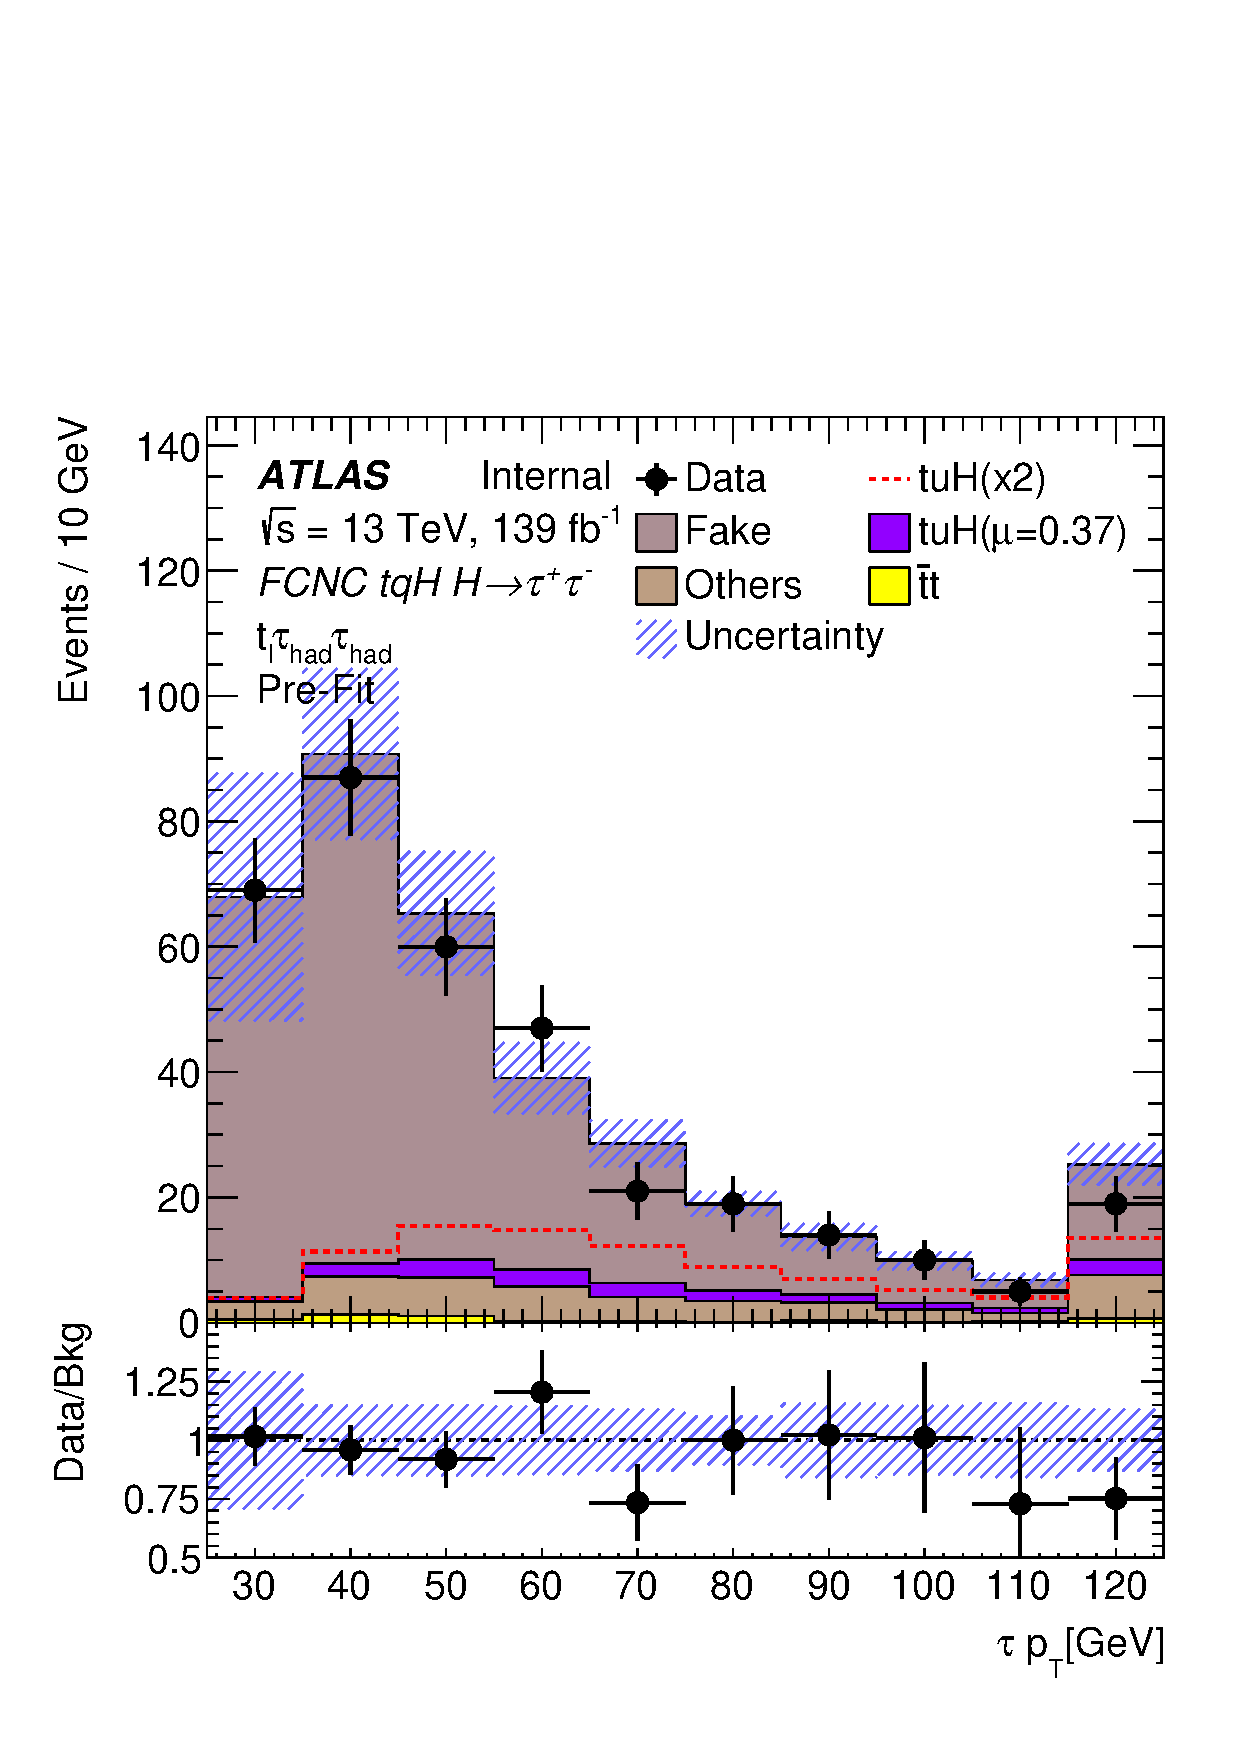
\includegraphics[page=1,width=0.33\textwidth]{figures/new_pt/reg1l2tau1bnj_os.pdf} &
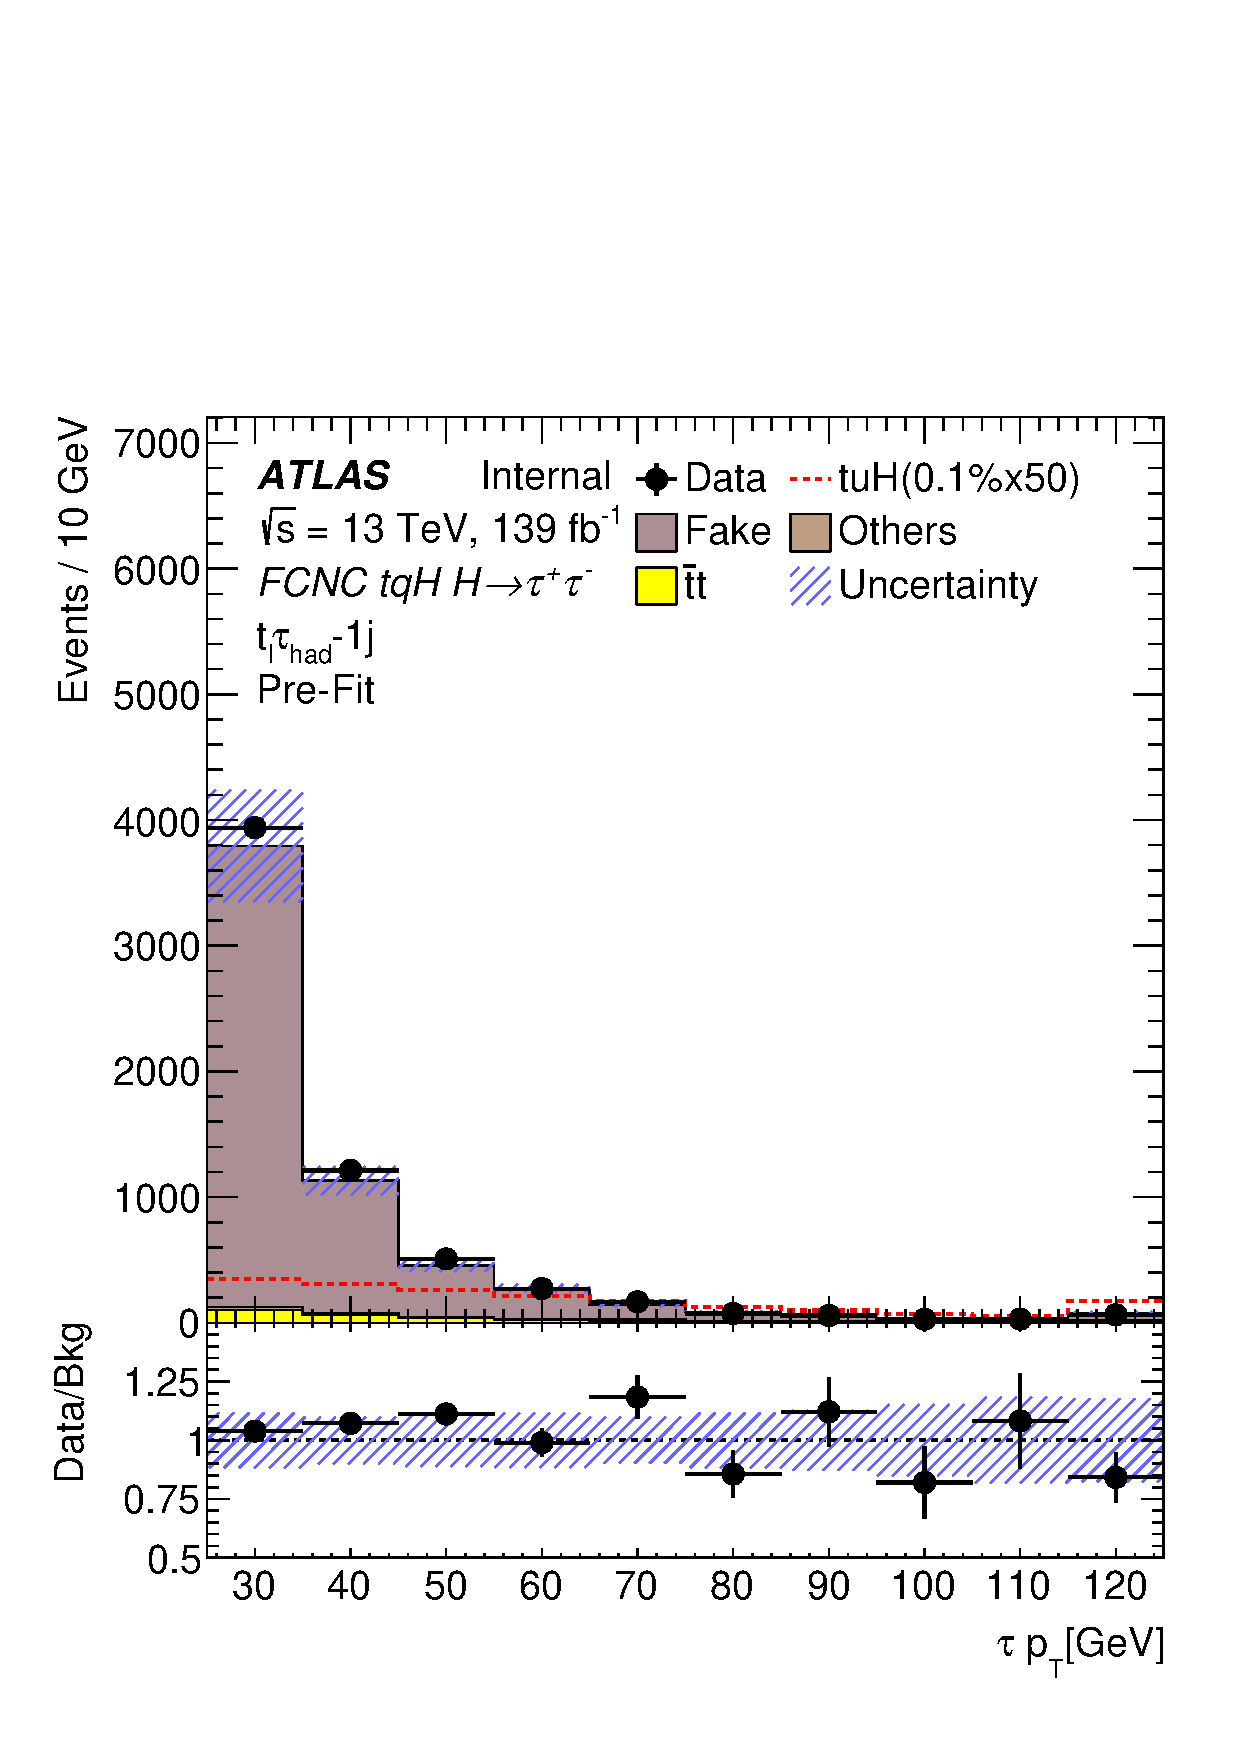
\includegraphics[page=1,width=0.33\textwidth]{figures/new_pt/reg1l1tau1b1j_ss.pdf}&
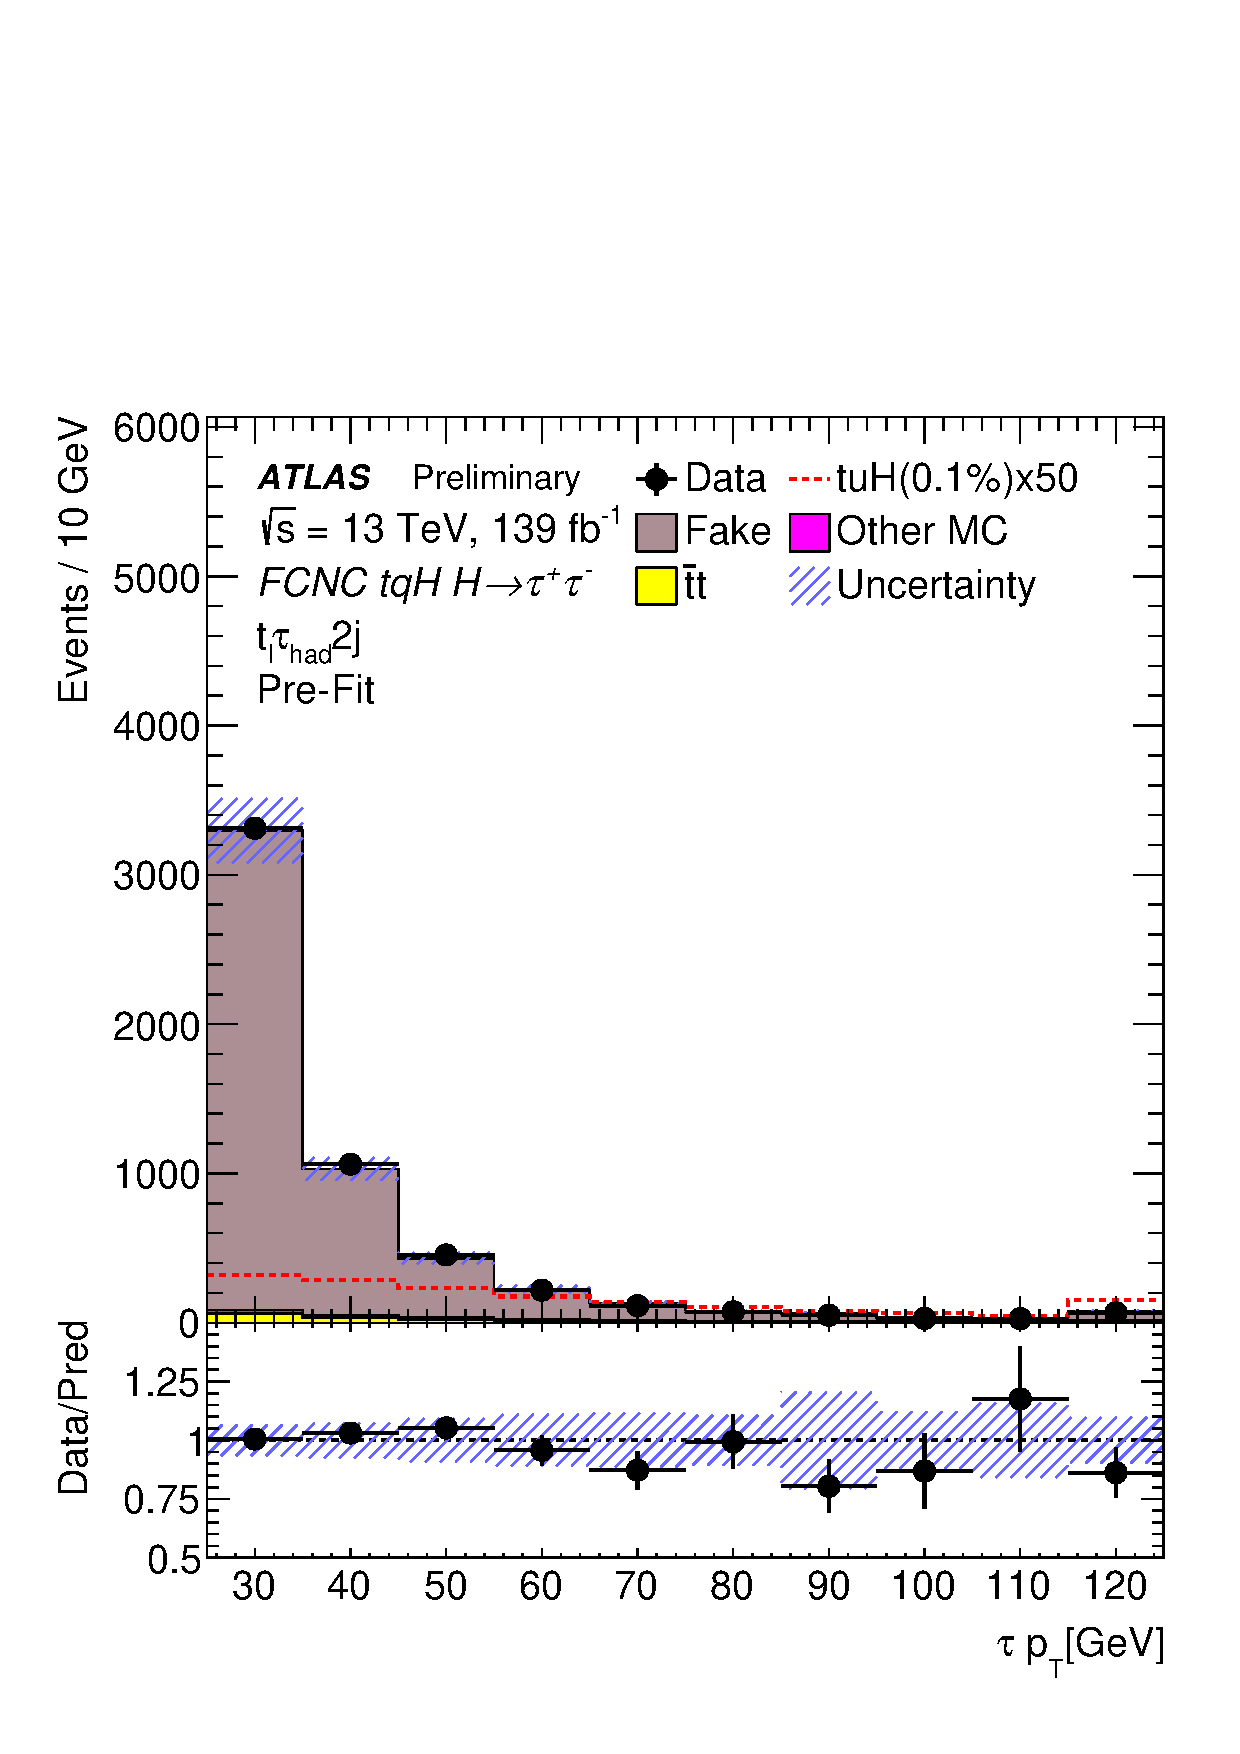
\includegraphics[page=1,width=0.33\textwidth]{figures/new_pt/reg1l1tau1b2j_ss.pdf}\\
(a) & (b) & (c) \\
%(a1) \pT(\tauhad) in $t_{\ell}\thadhad$ & (a2) \pT(\tauhad) in  $t_{\ell}\tauhad$-1j& (a3) \pT(\tauhad) in $t_{\ell}\tauhad$-2j\\
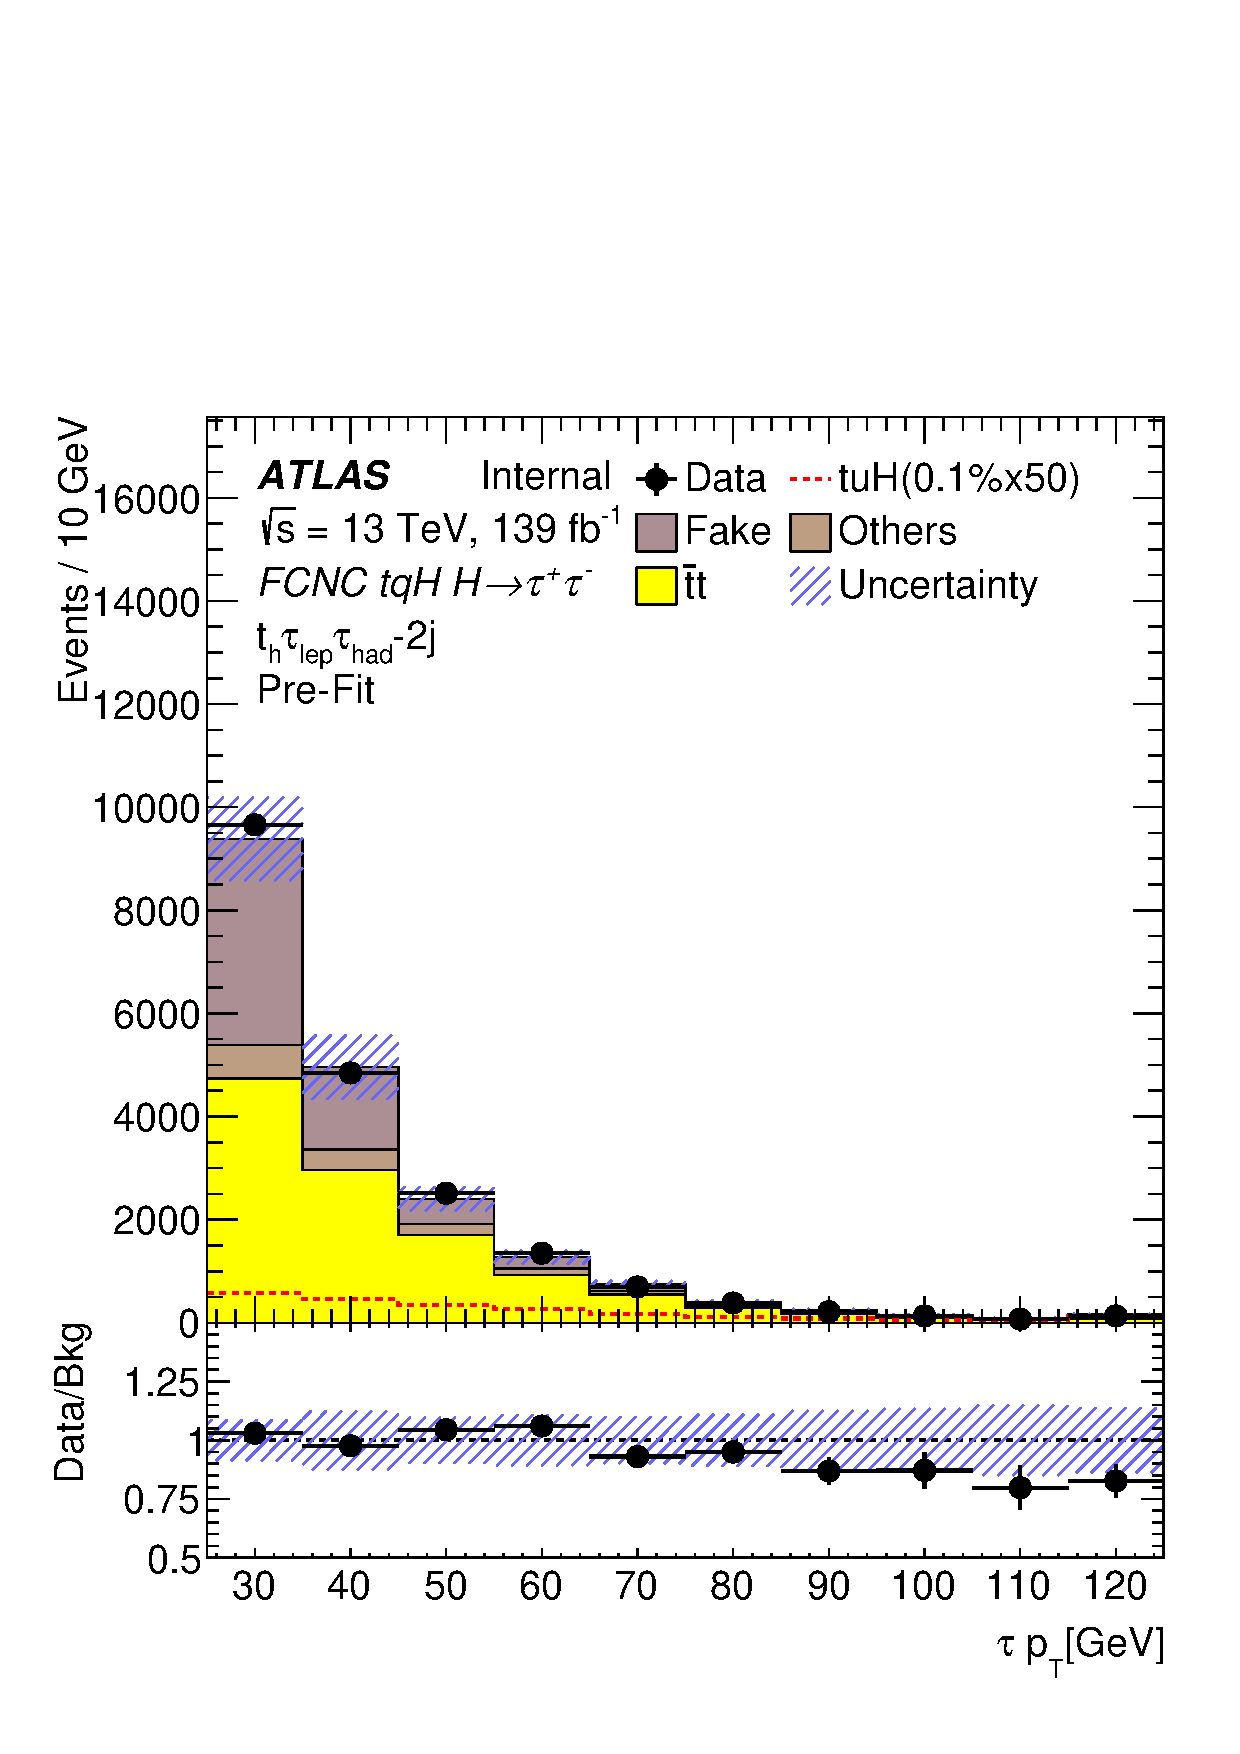
\includegraphics[page=1,width=0.33\textwidth]{figures/new_pt/reg1l1tau1b2j_os.pdf}&
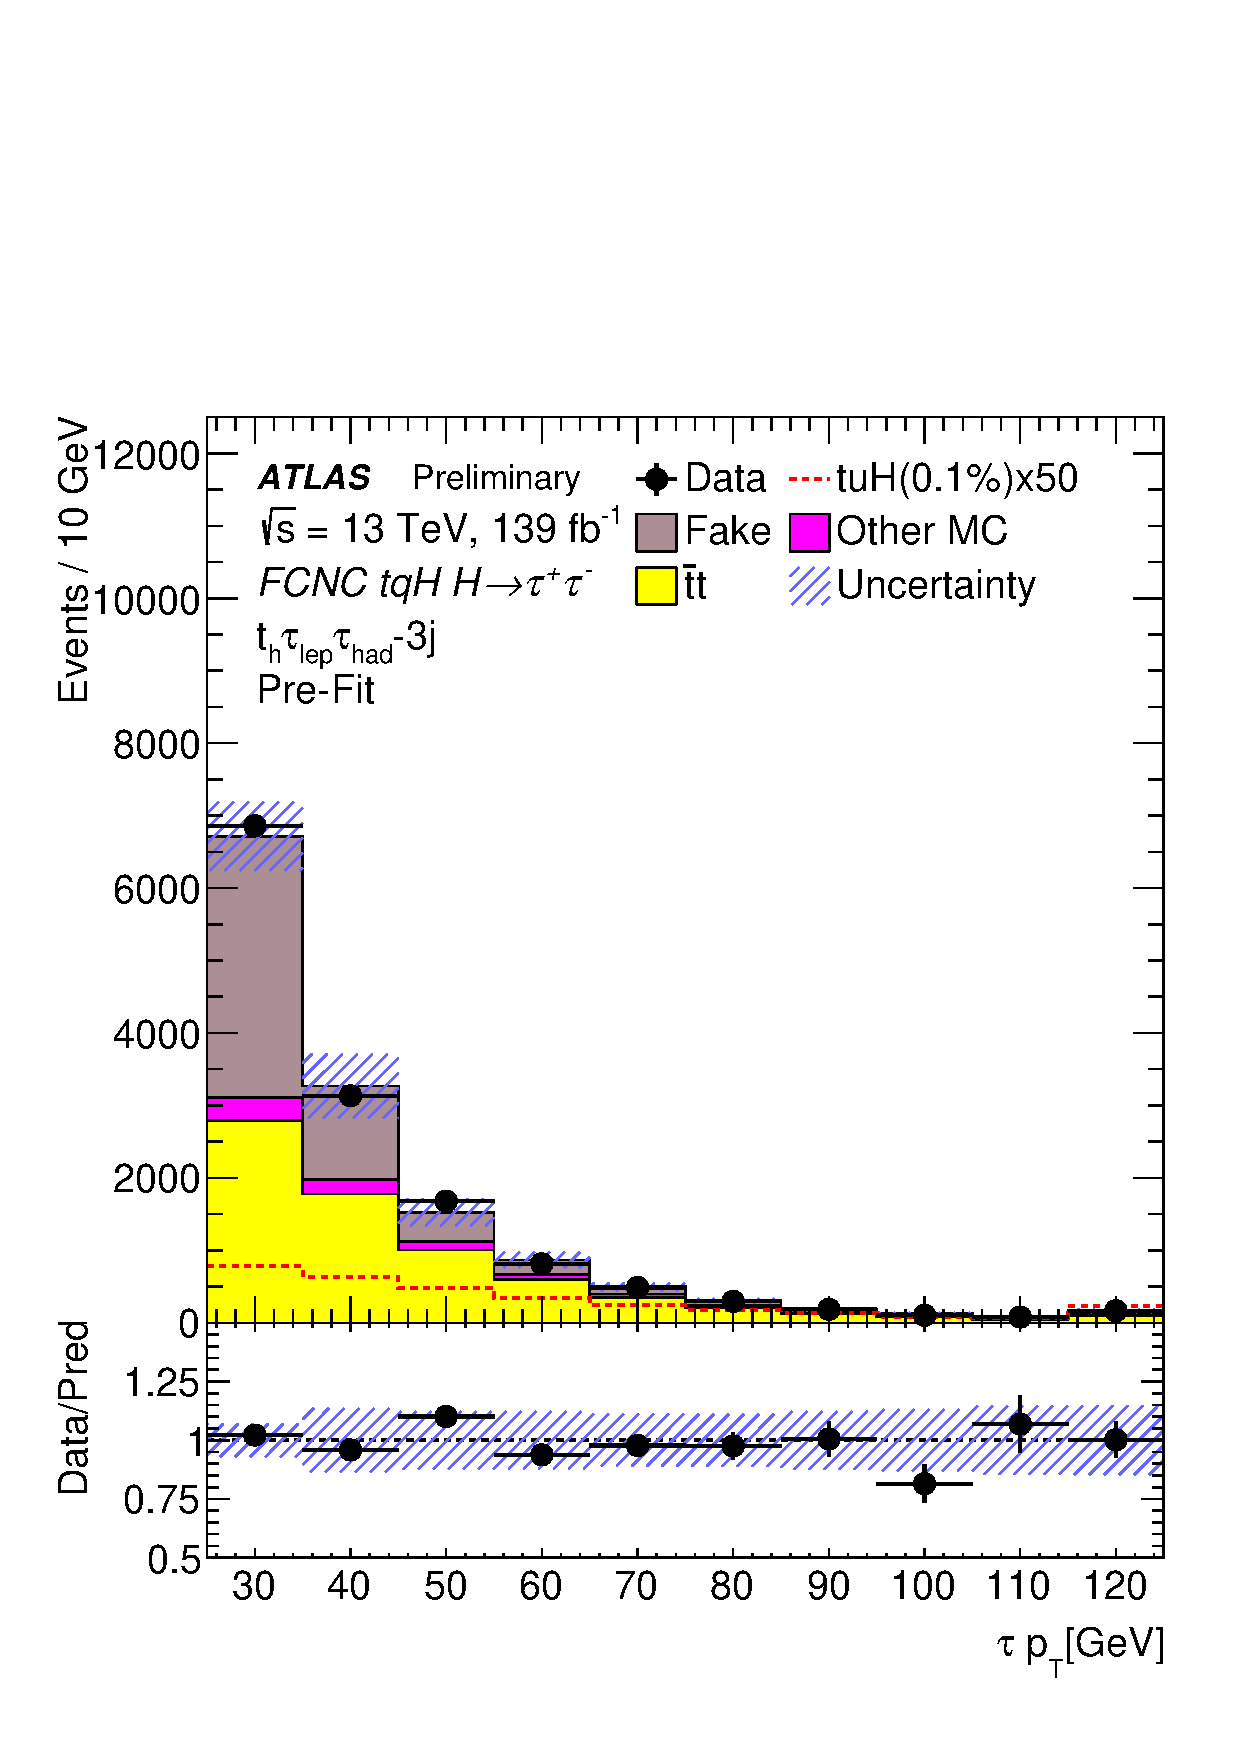
\includegraphics[page=1,width=0.33\textwidth]{figures/new_pt/reg1l1tau1b3j_os.pdf}\\
(d) & (e) \\
%(b1) \pT(\tauhad) in $t_h\tlhad$-2j & (b2) \pT(\tauhad) in  $t_h\tlhad$-3j & (b3) \pT(\tauhad) in $t_h\thadhad$-2j \\
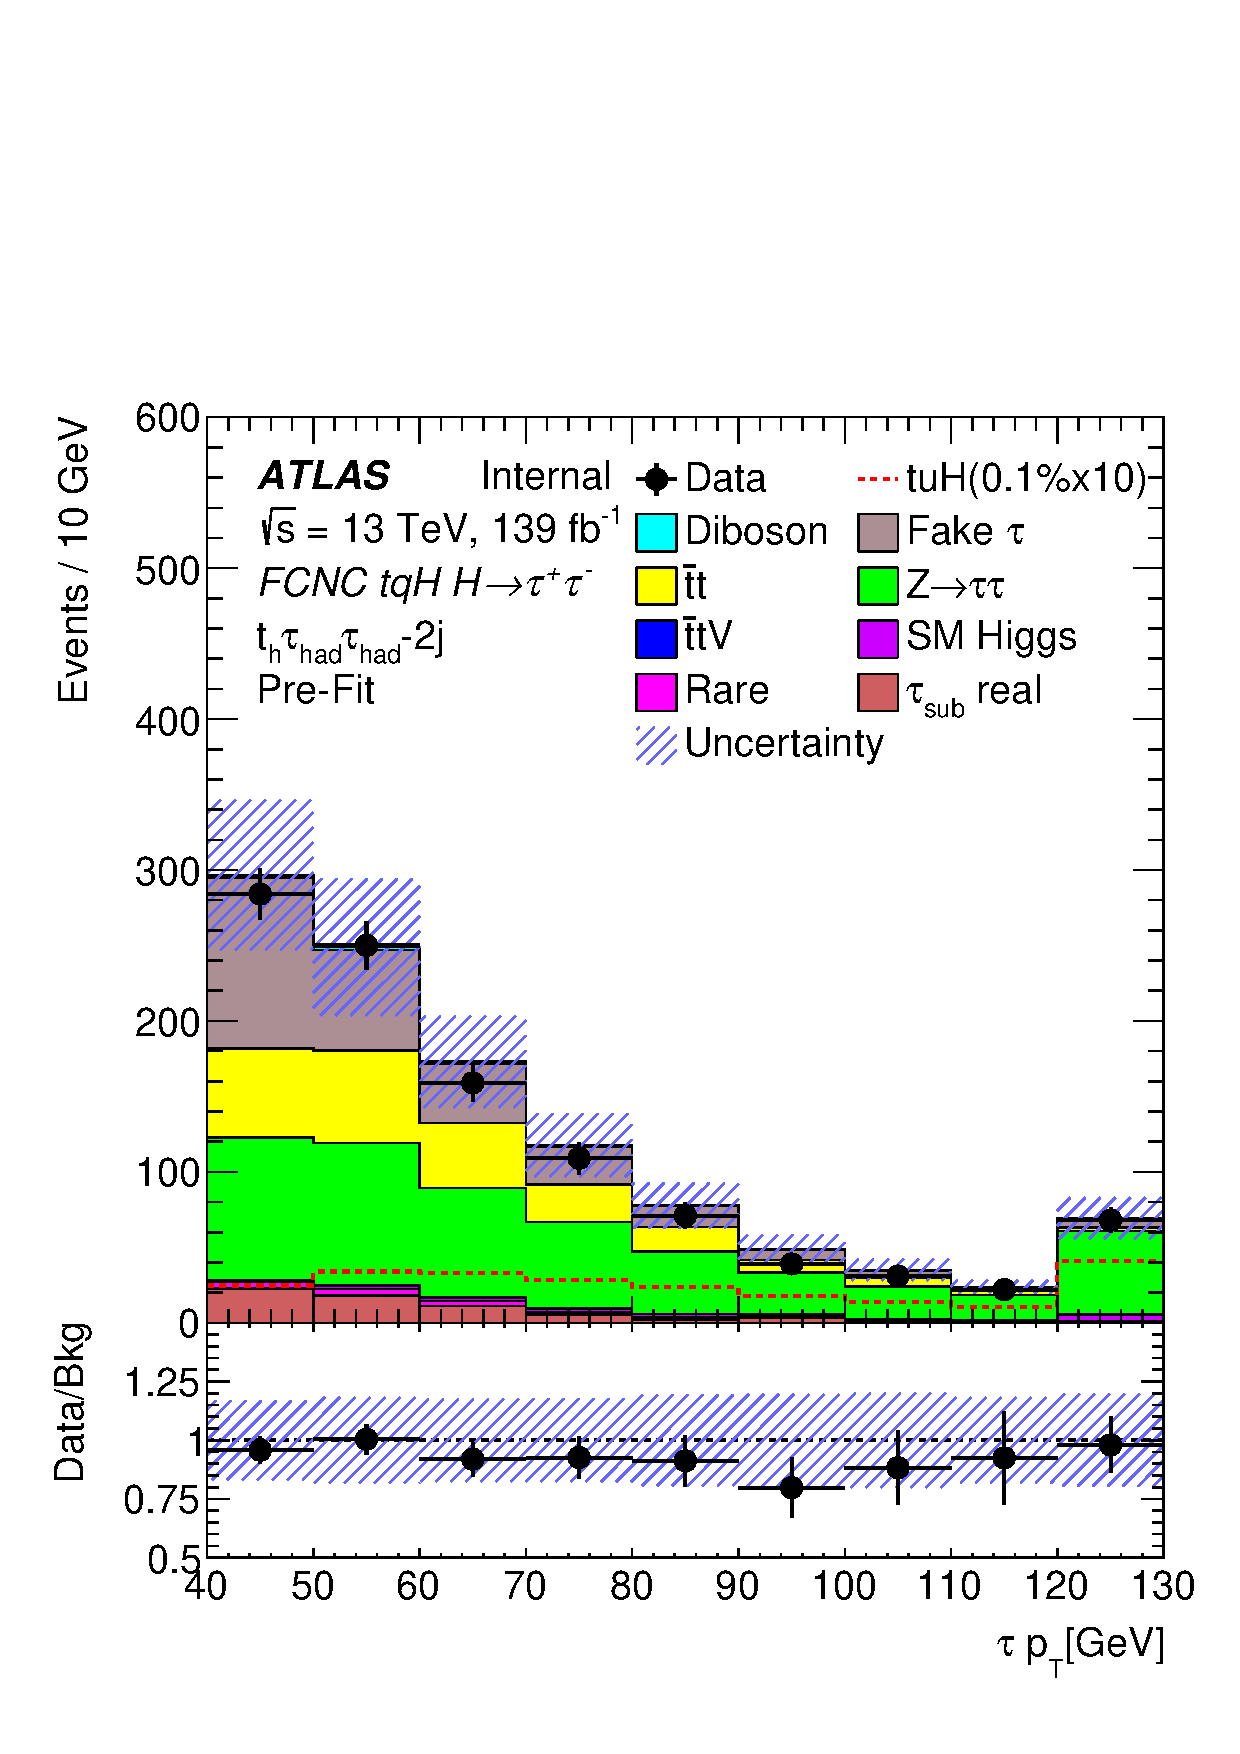
\includegraphics[page=1,width=0.33\textwidth]{figures/new_pt/reg2mtau1b2jos_vetobtagwp70_highmet.pdf}&
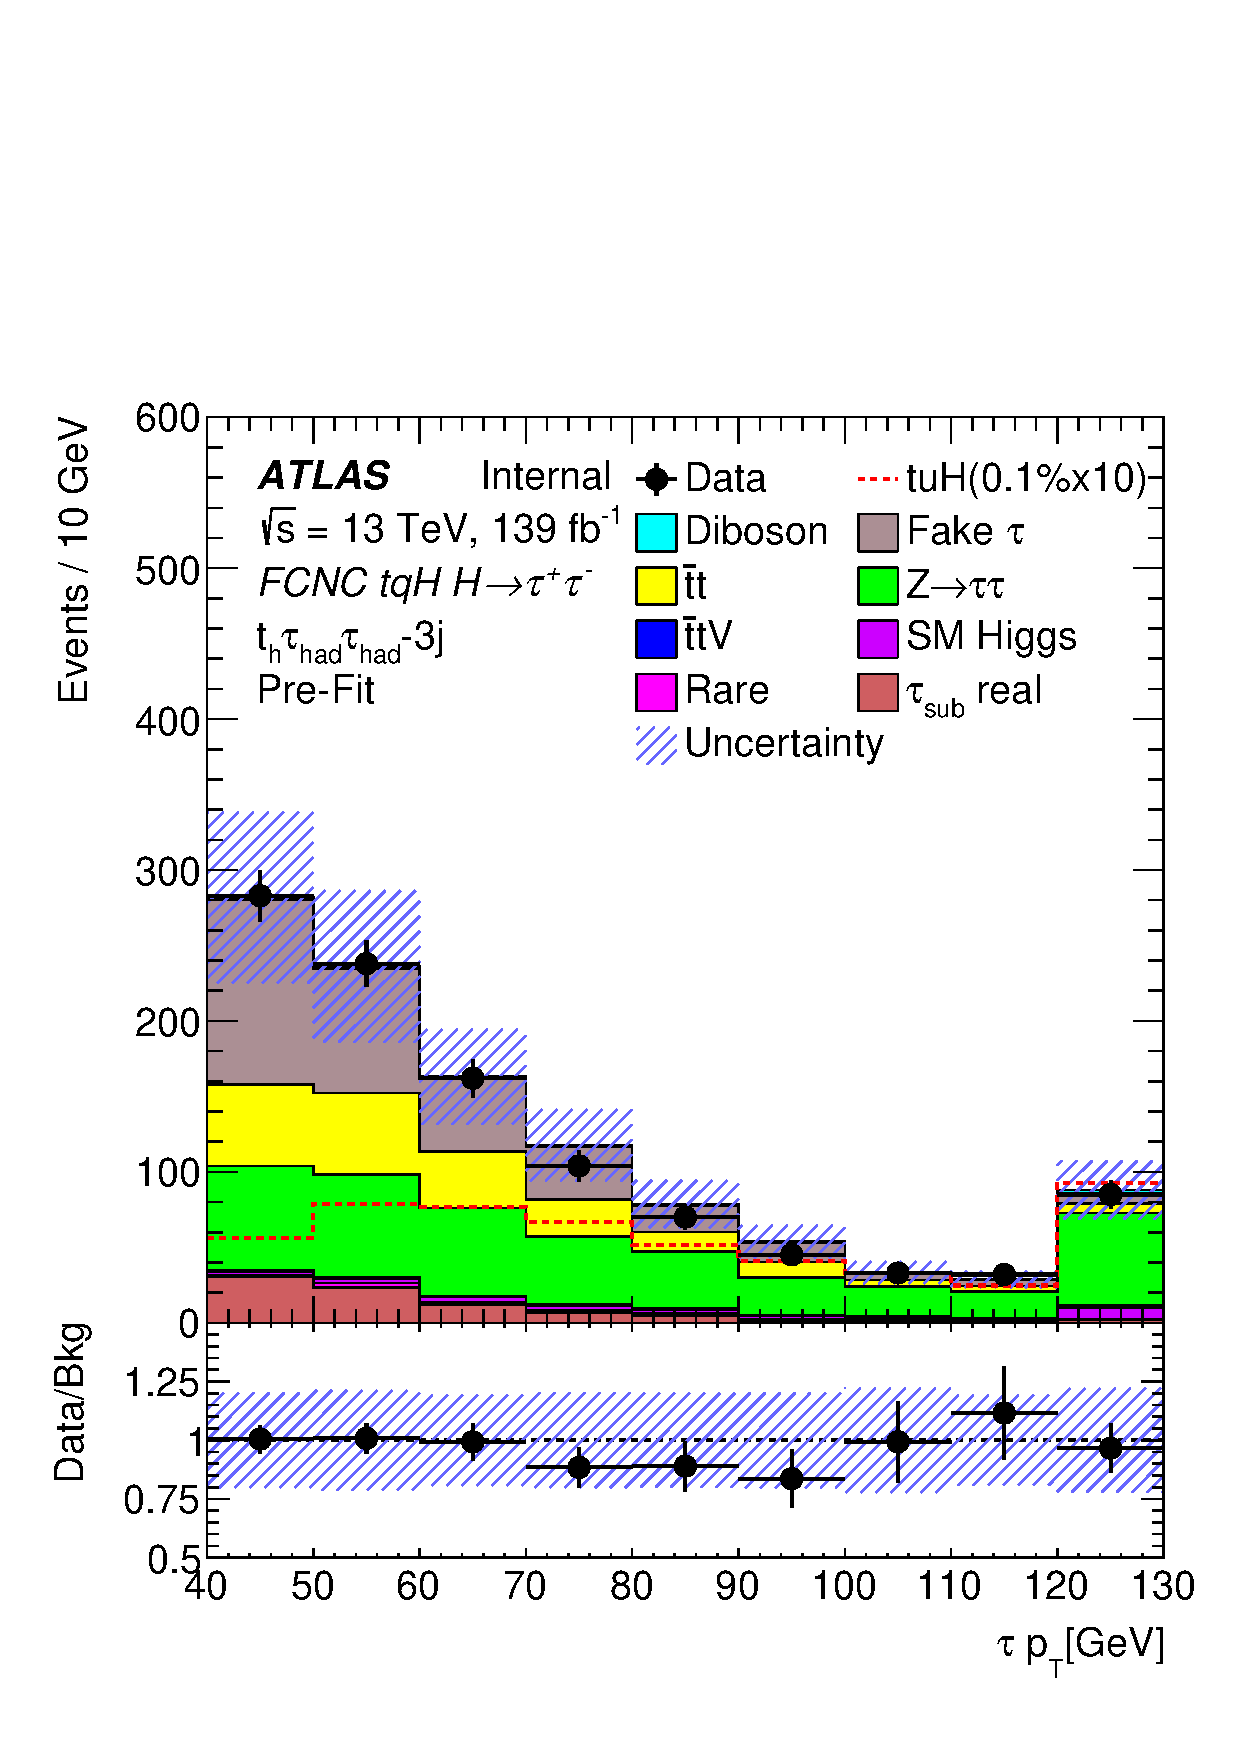
\includegraphics[page=1,width=0.33\textwidth]{figures/new_pt/reg2mtau1b3jos_vetobtagwp70_highmet.pdf}\\
(f) & (g) \\
%(c1) \pT(\tauhad) in $t_h\thadhad$-3j\\
\end{tabular}
\caption{Leading $\thad$ $\pt$  distributions obtained before the fit to data ('Pre-Fit') showing 
  the expected background and $tuH$ signals after applying fake factors in the following SRs: $t_{\ell}\thadhad$ (a),
  $t_{\ell}\tauhad$-1j (b),  $t_{\ell}\tauhad$-2j (c), $t_h\tlhad$-2j (d), $t_h\tlhad$-3j (e), $t_h\thadhad$-2j (f), and $t_h\thadhad$-3j (g).
 The total size of the statistical and systematic uncertainties of the background prediction is indicated by the hatched band.
 %The uncertainty band includes both the statistical and systematic uncertainties in the background prediction.
 Overflow events are included in the last bin. ``Other MC'' (``Rare'') includes single top, and $V$+jets and other small backgrounds in the leptonic (hadronic) channel. The $tuH$ signal is scaled using a normalization factor of 2 to 50.   
%( only subtau real refers to $t\bar{t}$ MC with leading tau faked by other object, subleading tau from real contribution. 
The lower panels show the data to prediction ratio.}
\label{fig:taupt_prefit}
\end{figure}









% \begin{figure}[H]
% \centering
% 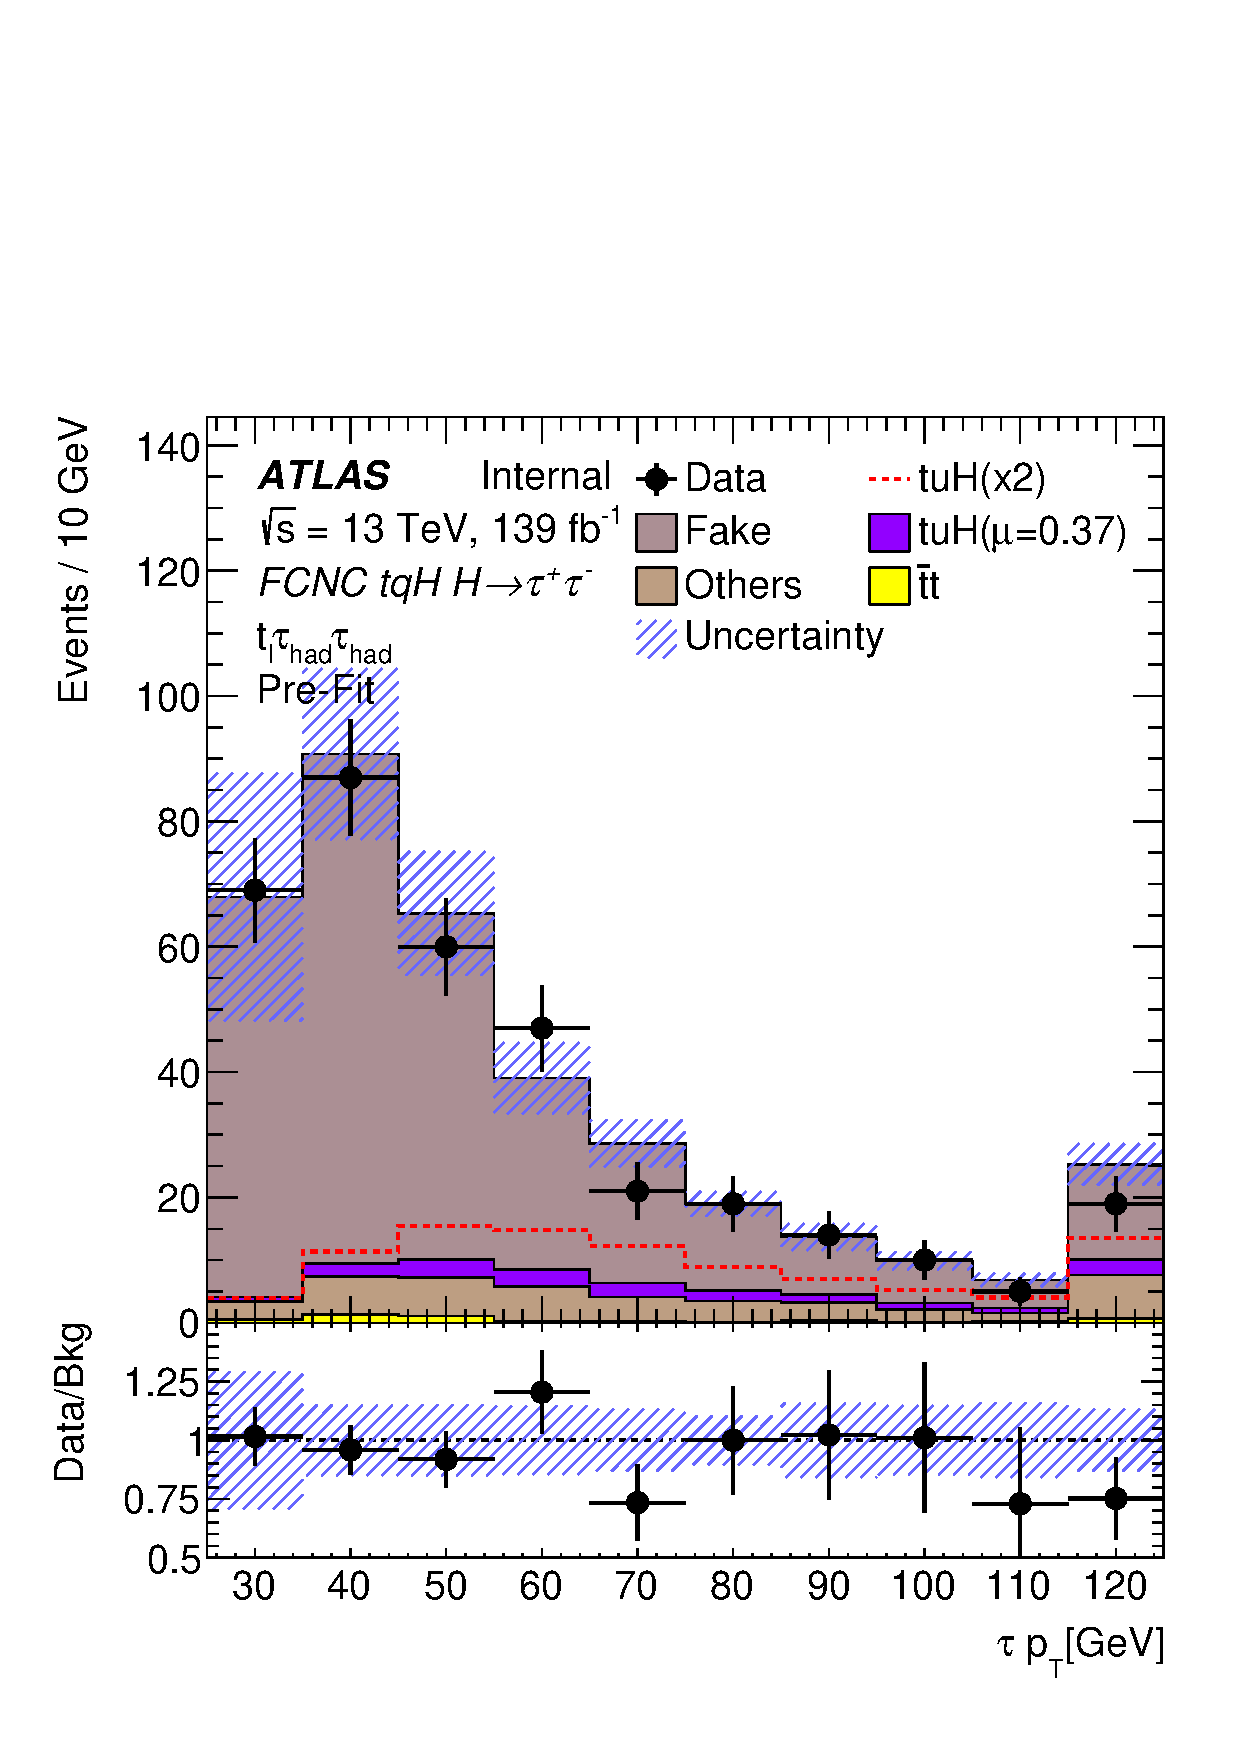
\includegraphics[width=0.31\textwidth]{figures/new_pt/reg1l2tau1bnj_os.pdf}
% 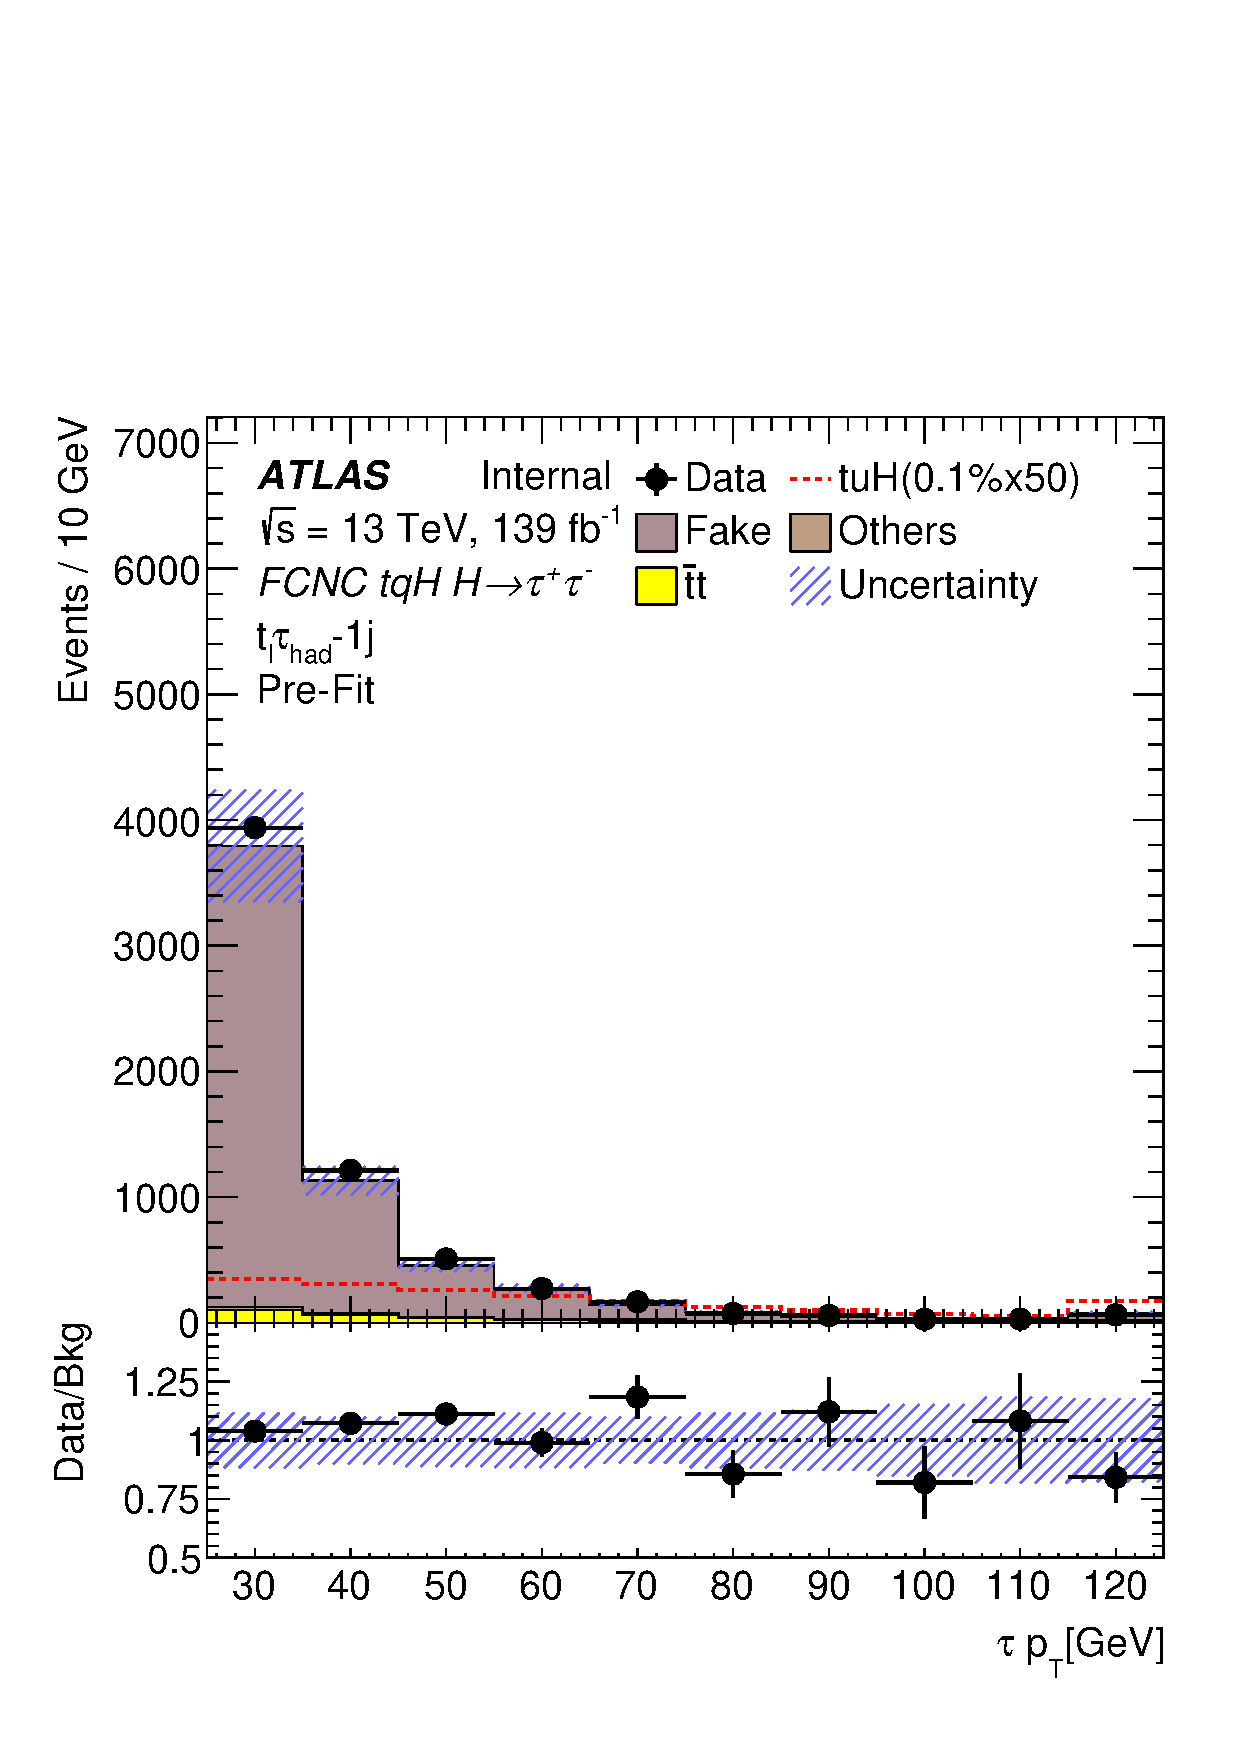
\includegraphics[width=0.31\textwidth]{figures/new_pt/reg1l1tau1b1j_ss.pdf}
% 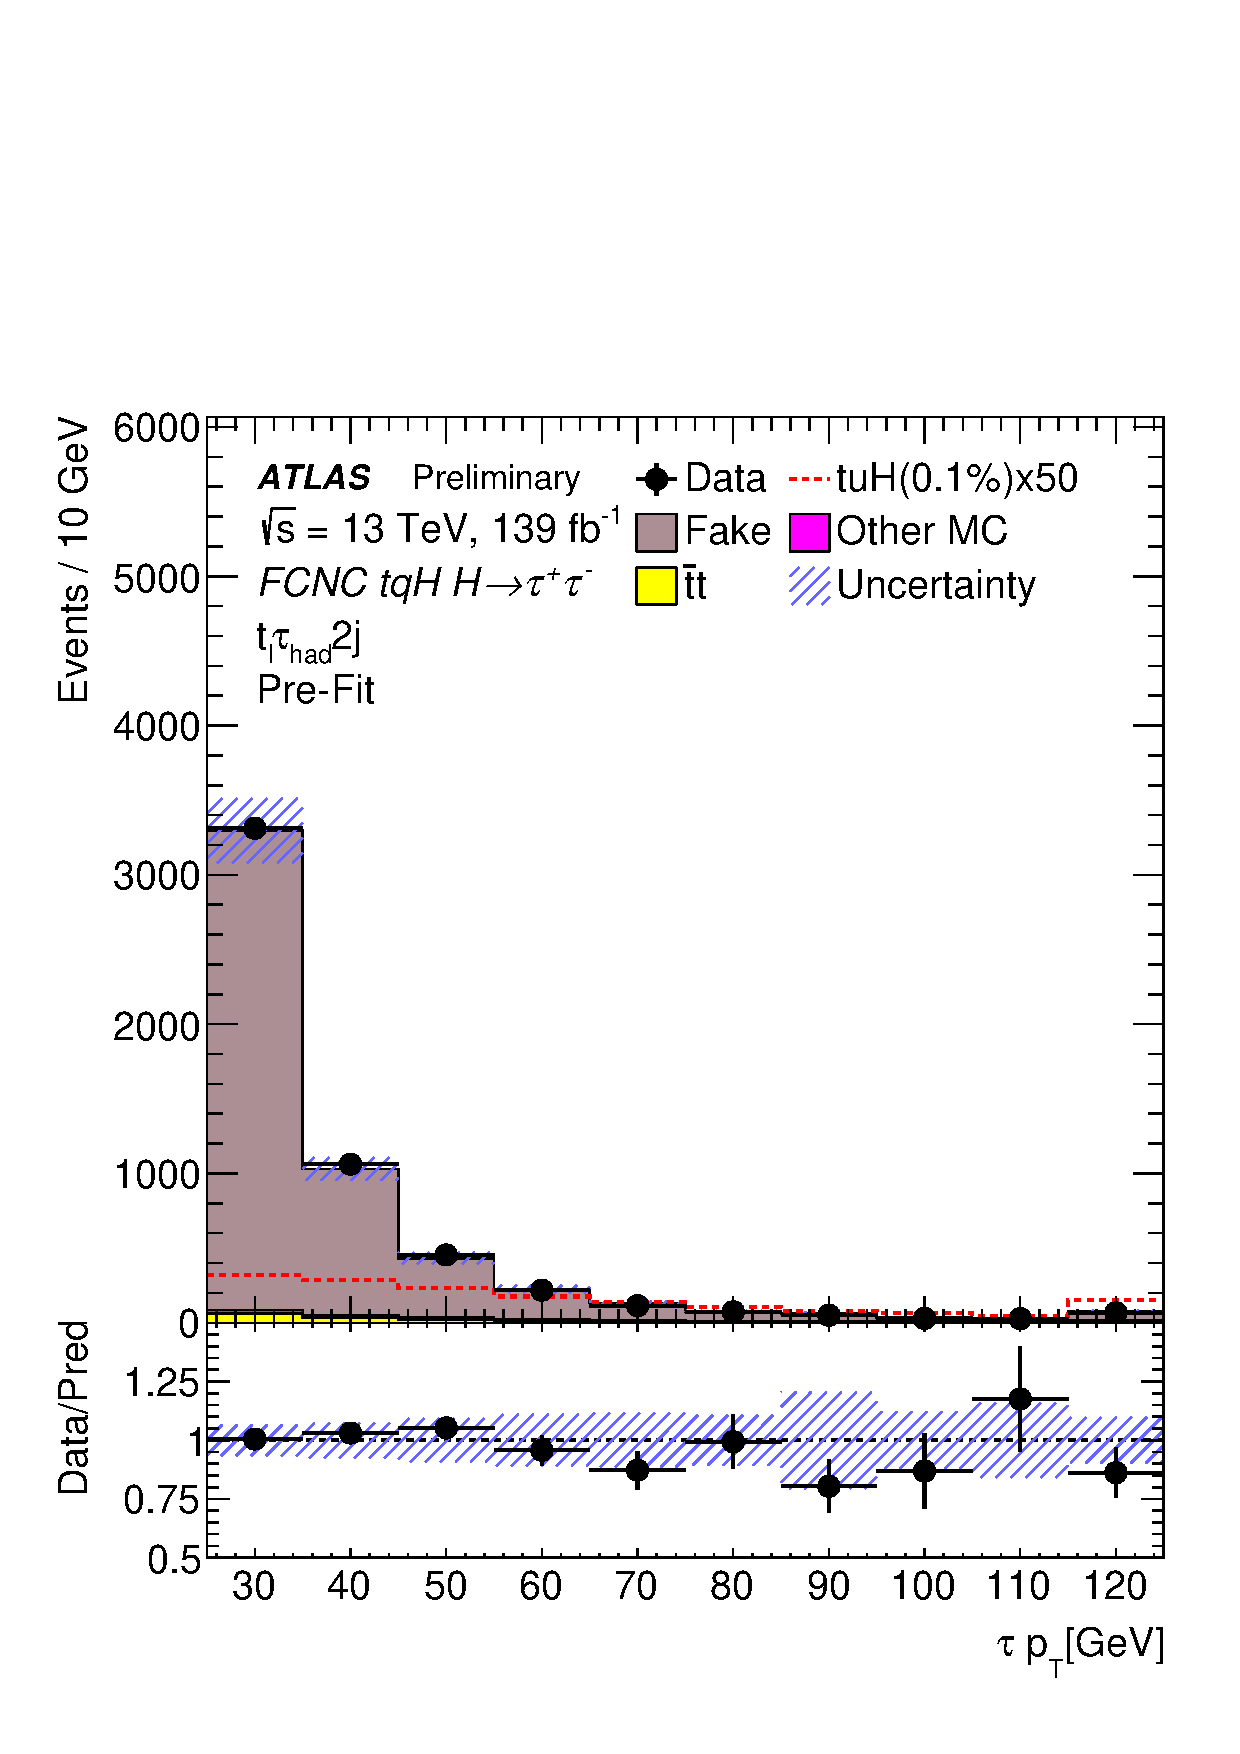
\includegraphics[width=0.31\textwidth]{figures/new_pt/reg1l1tau1b2j_ss.pdf}\\
% (a1)  (a2)  (a3) \\
% 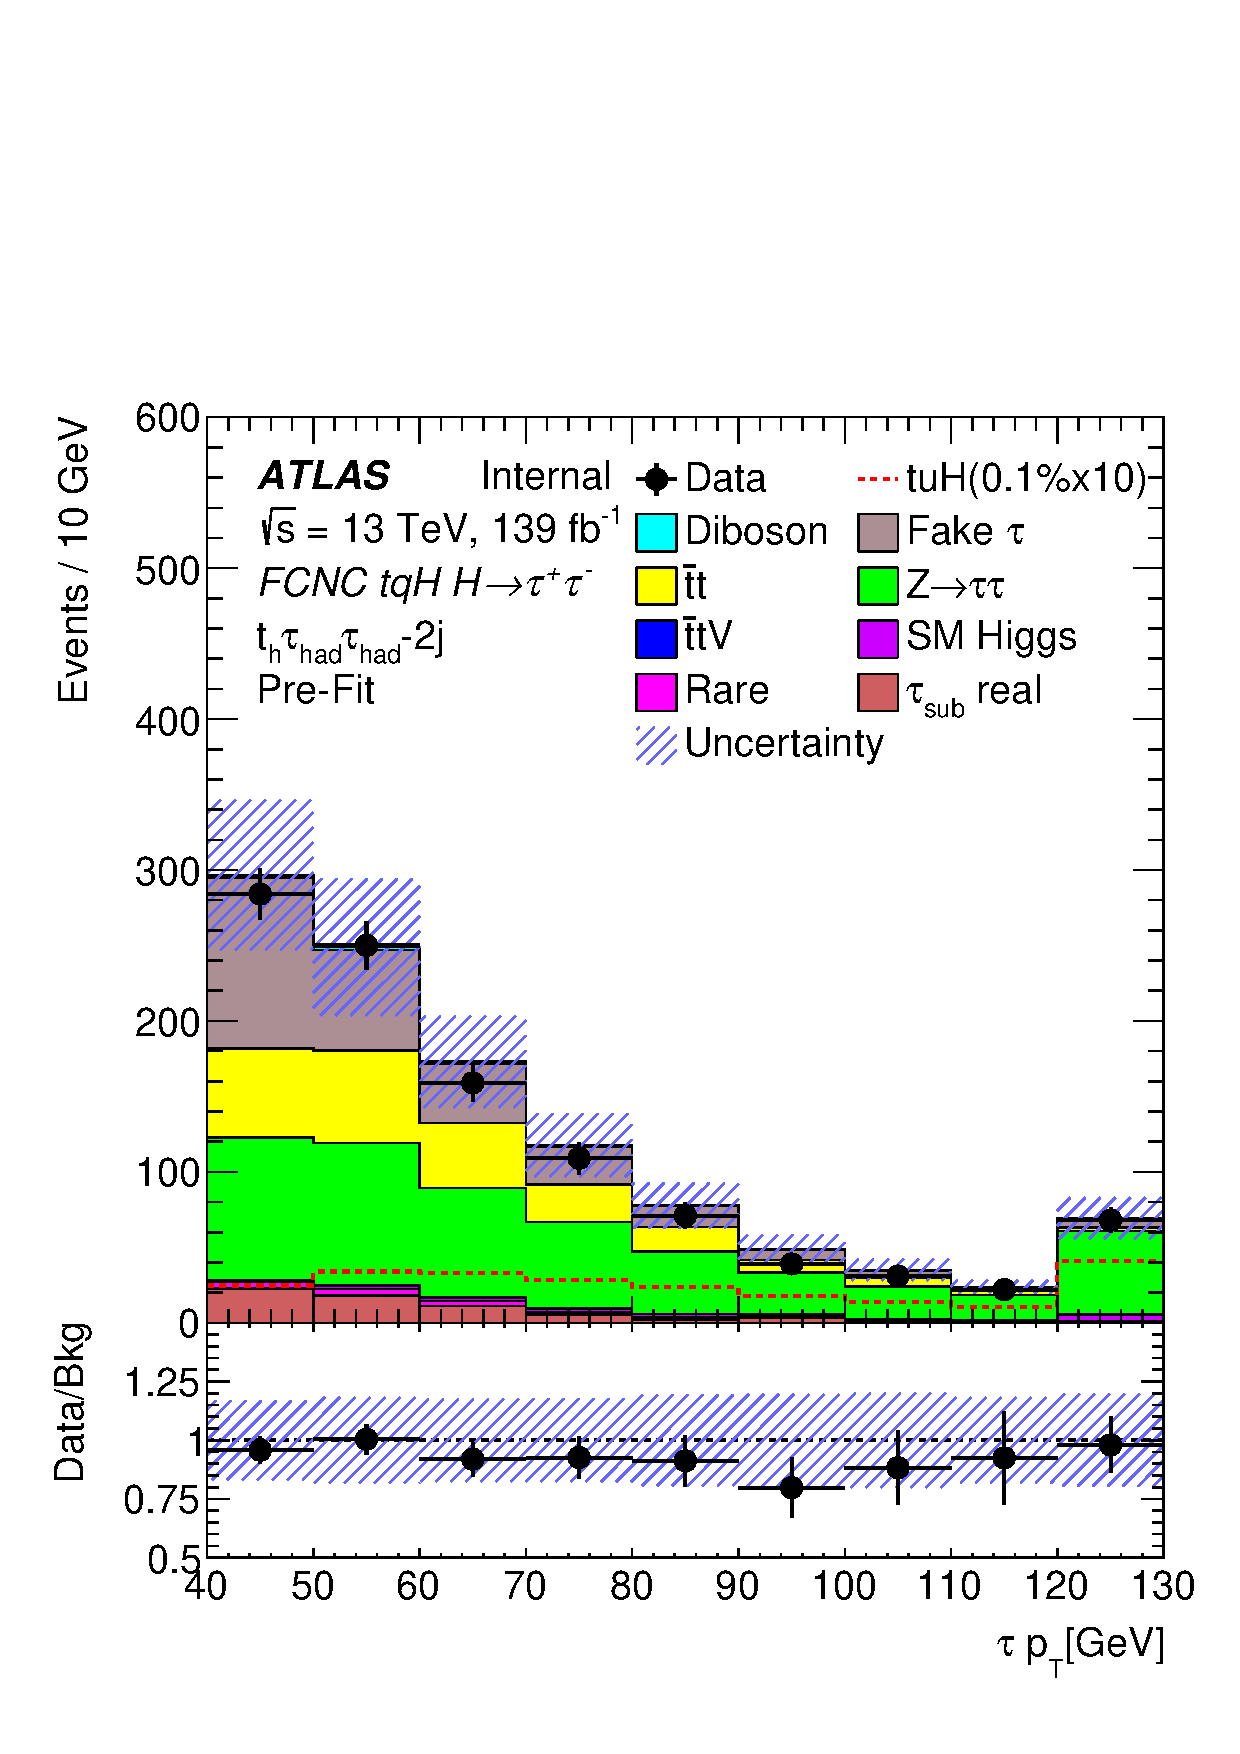
\includegraphics[width=0.31\textwidth]{figures/new_pt/reg2mtau1b2jos_vetobtagwp70_highmet.pdf}
% 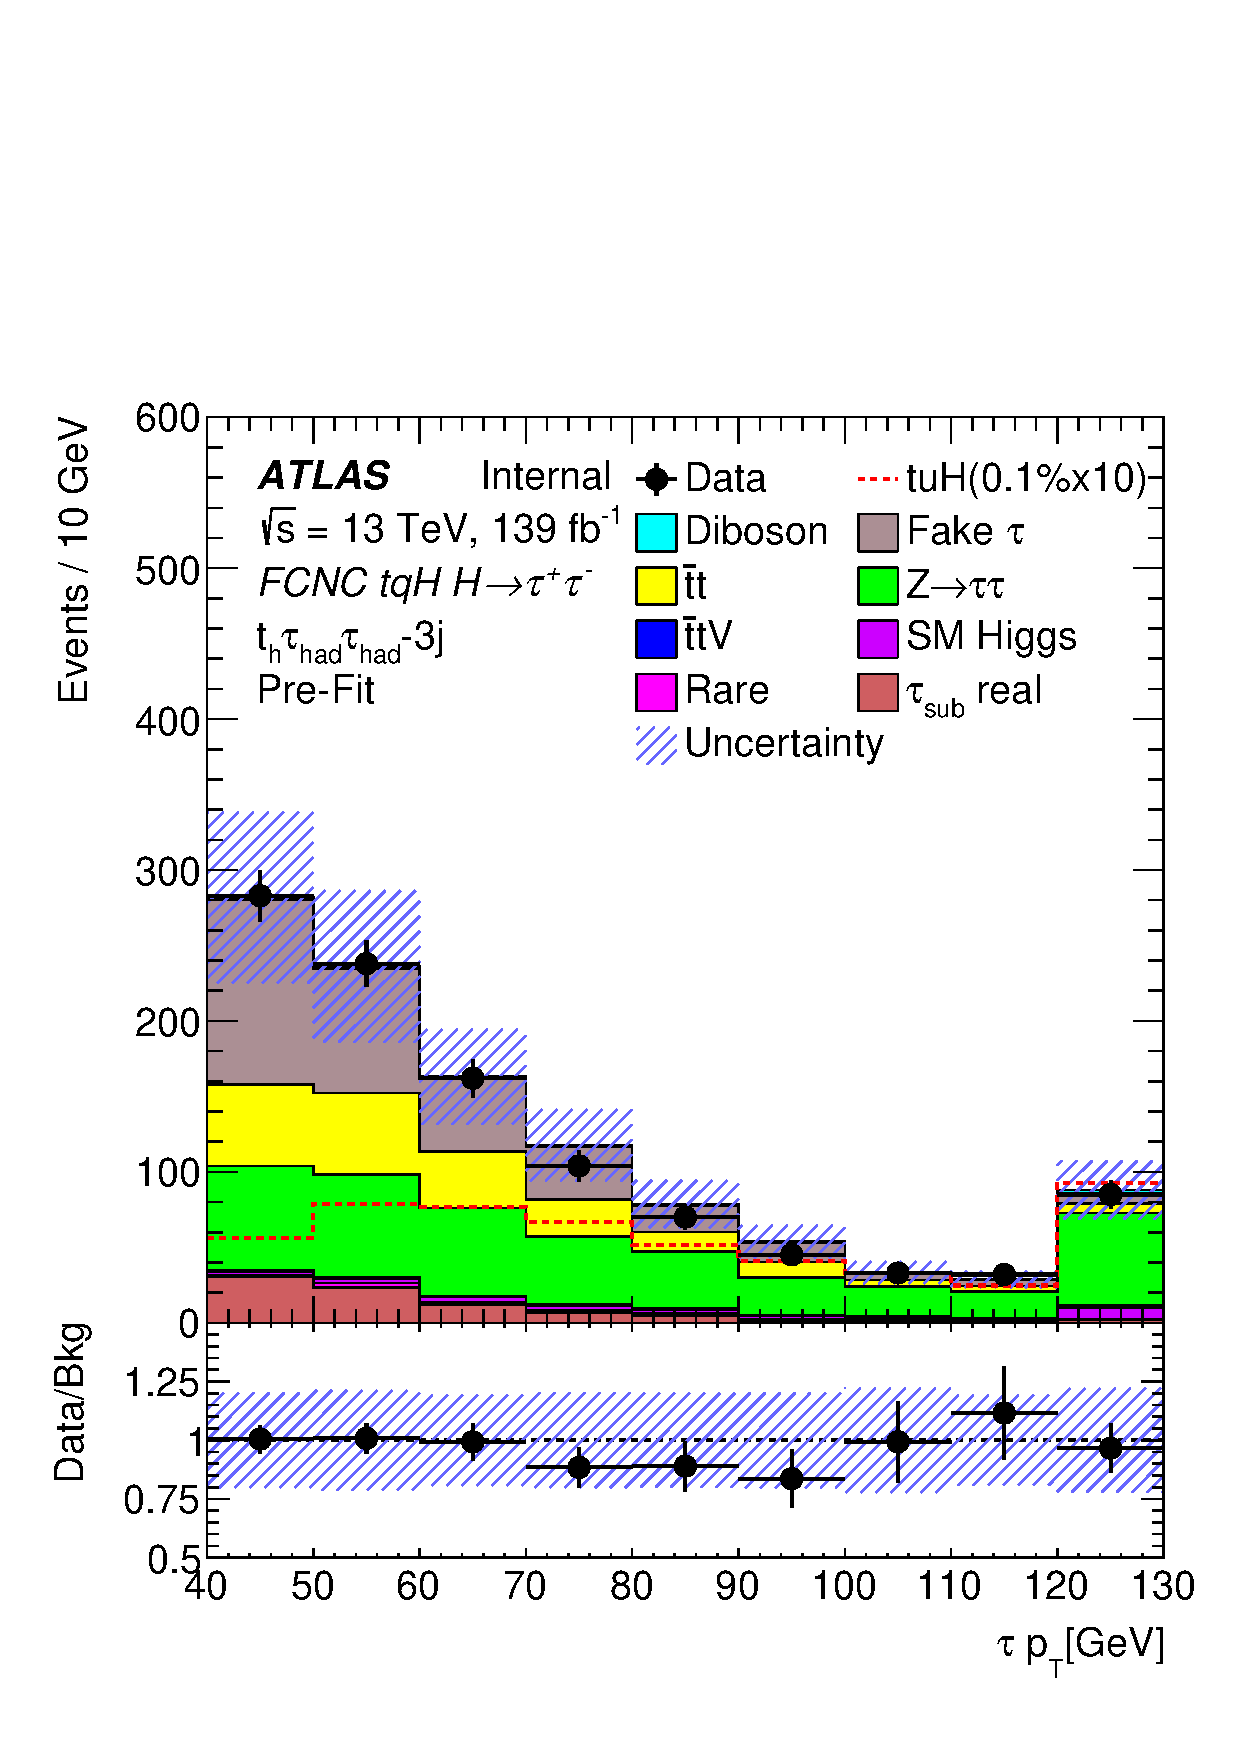
\includegraphics[width=0.31\textwidth]{figures/new_pt/reg2mtau1b3jos_vetobtagwp70_highmet.pdf} \\ 
% (a1)  (a2)  (a3) \\
% 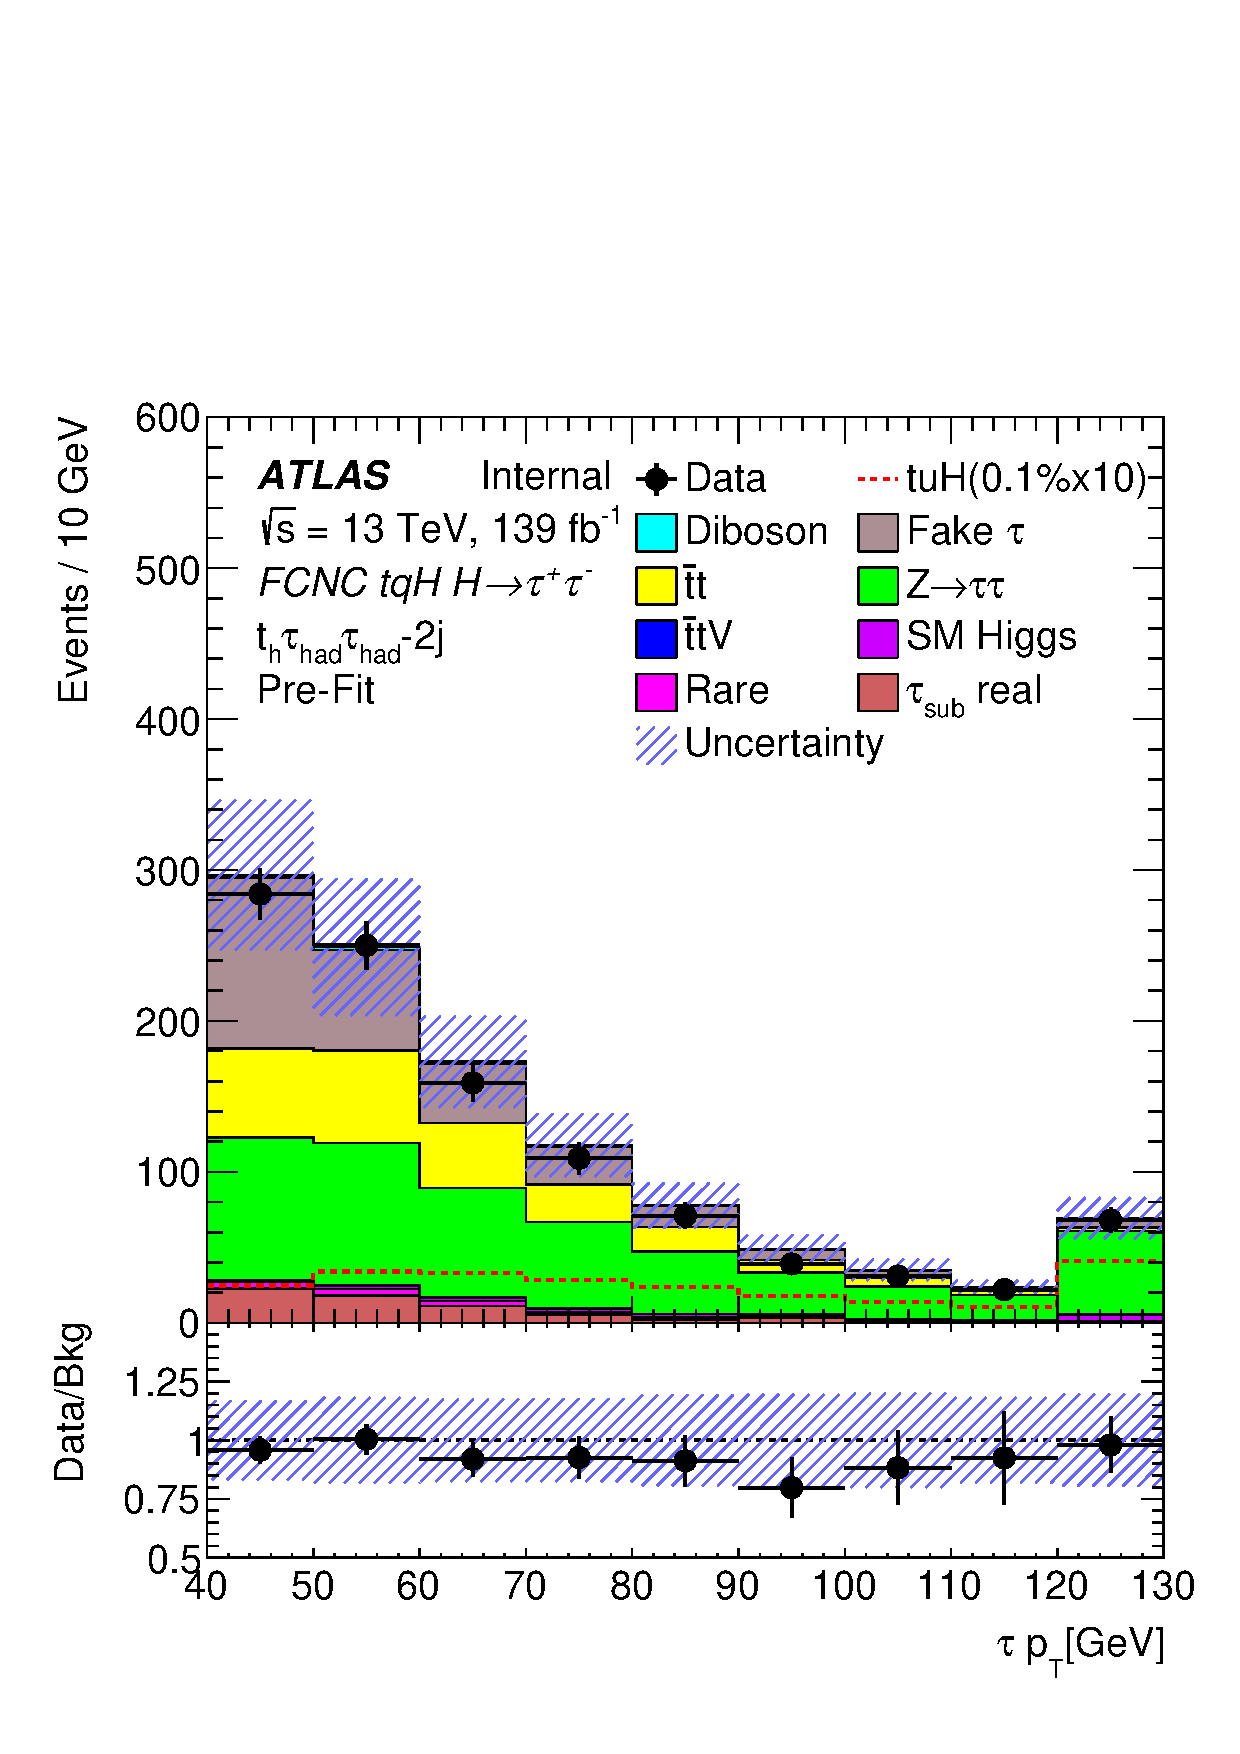
\includegraphics[width=0.31\textwidth]{figures/new_pt/reg2mtau1b2jos_vetobtagwp70_highmet.pdf}
% 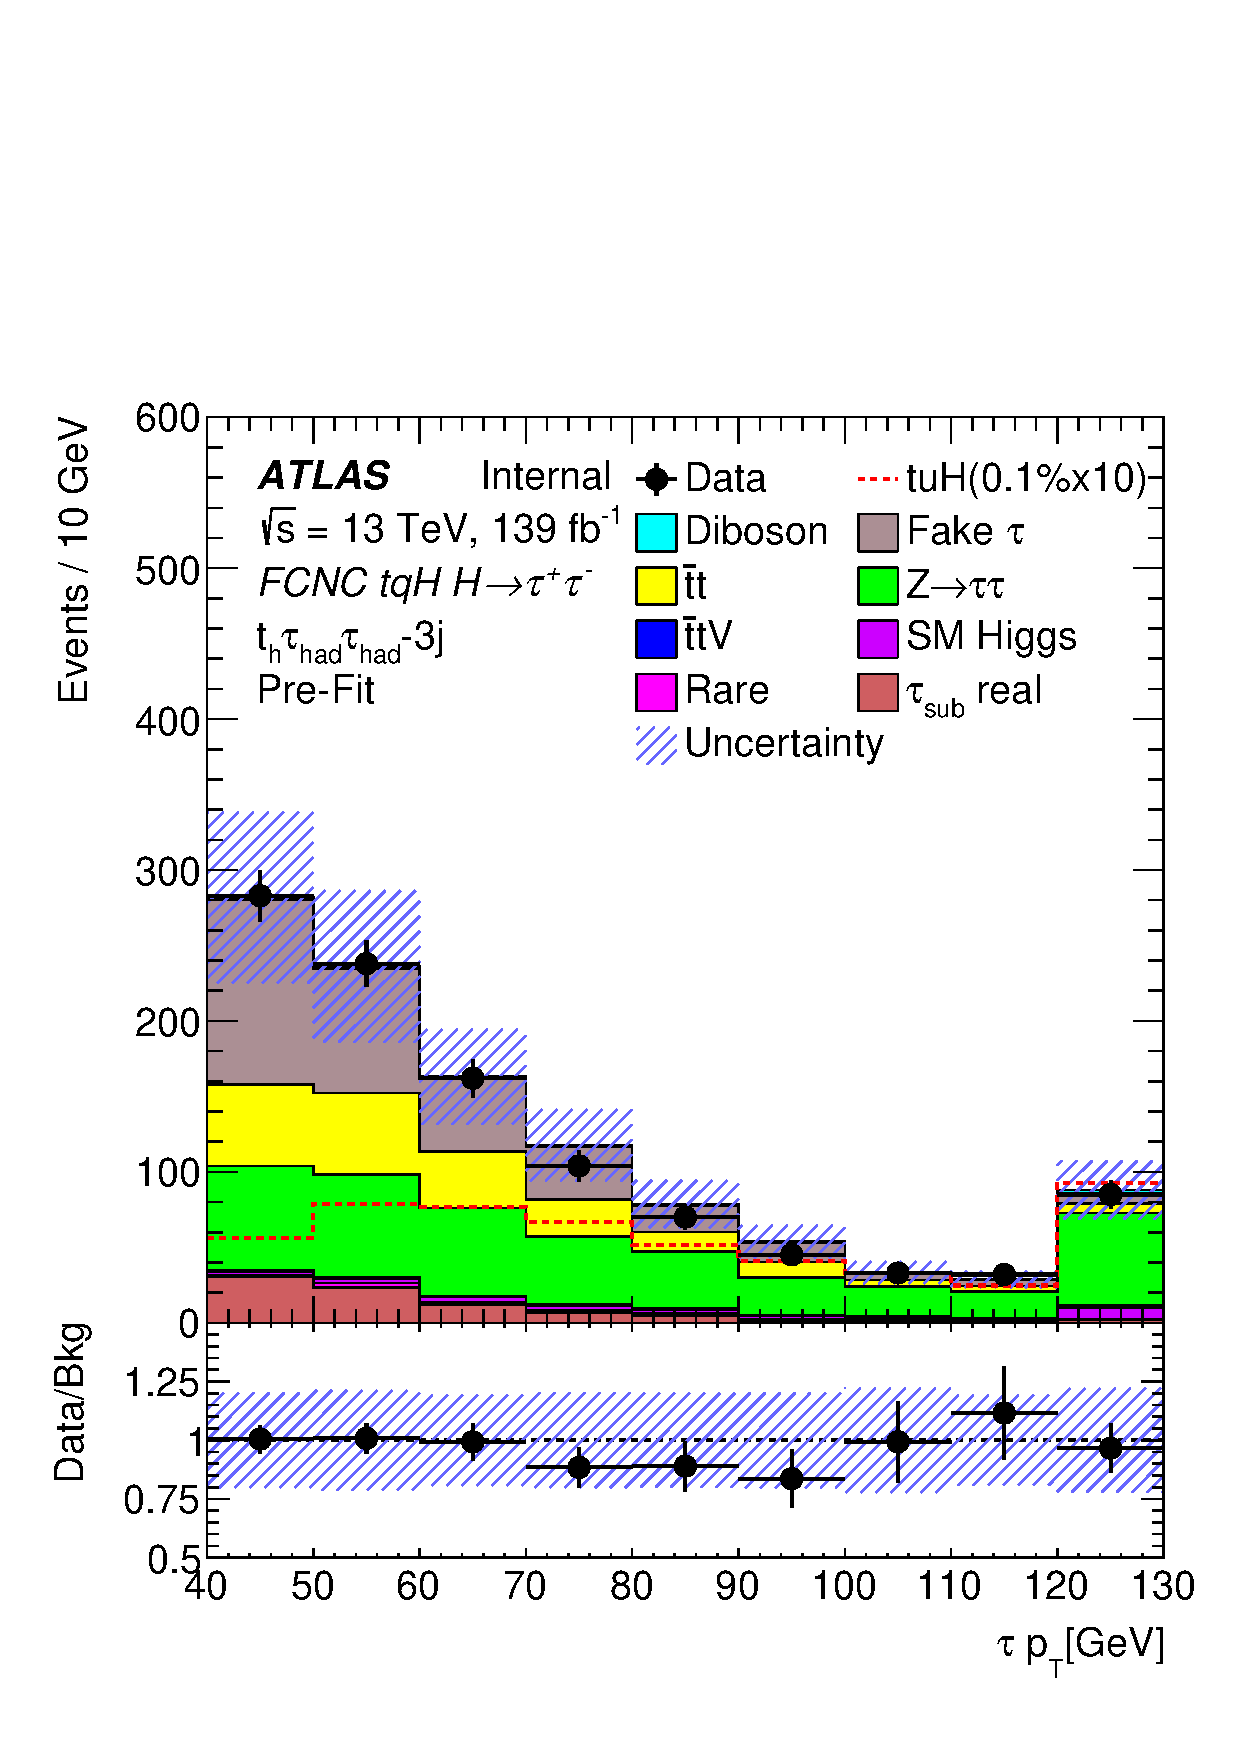
\includegraphics[width=0.31\textwidth]{figures/new_pt/reg2mtau1b3jos_vetobtagwp70_highmet.pdf} \\ 
% (a1)  (a2)  (a3) \\
% \caption{ The BDT output distributions for the background and TT signal (a1, b1), background and ST signal (a2, b2), background and different types of signals (c1,c2) and % ROC curves (a3, b3) in the $t_h\thadhad$-2j (a1-3,c1), $t_h\thadhad$-3j (b1-3,c2) regions of leptonic channel. Only statistical uncertainties are being shown. Underflow % and overflow bins are included respectively in the first and last bins. The real tau contributions shown from various MC samples.}% The Kolmogorov Test values for the % training and testing BDT distributions are also indicated.
% \label{fig:overtrain_hadhad}
% \end{figure}



















% %\input{\FCNCFigures/tex/BDT}
% \begin{figure}[H]
% \centering
% \begin{tabular}{@{}ccc@{}}
% \includegraphics[page=7,width=0.33\textwidth]{\FCNCFigures/tthML/showFake/faketau/postfit/NOMINAL_fancpaper/reg1l2tau1bnj_os/BDTG_test.pdf} &
% \includegraphics[page=7,width=0.33\textwidth]{\FCNCFigures/tthML/showFake/faketau/postfit/NOMINAL_fancpaper/reg1l1tau1b1j_ss_vetobtagwp70_highmet/BDTG_test.pdf}&
% \includegraphics[page=7,width=0.33\textwidth]{\FCNCFigures/tthML/showFake/faketau/postfit/NOMINAL_fancpaper/reg1l1tau1b2j_ss_vetobtagwp70_highmet/BDTG_test.pdf}\\
% (a1) BDT discriminant in $t_{\ell}\thadhad$ & (a2) BDT discriminant in  $t_{\ell}\tauhad$-1j& (a3) BDT discriminant in $t_{\ell}\tauhad$-2j\\
% \includegraphics[page=7,width=0.33\textwidth]{\FCNCFigures/tthML/showFake/faketau/postfit/NOMINAL_fancpaper/reg1l1tau1b2j_os_vetobtagwp70_highmet/BDTG_test.pdf} &
% \includegraphics[page=7,width=0.33\textwidth]{\FCNCFigures/tthML/showFake/faketau/postfit/NOMINAL_fancpaper/reg1l1tau1b3j_os_vetobtagwp70_highmet/BDTG_test.pdf} &
% \includegraphics[page=7,width=0.33\textwidth]{\FCNCFigures/xTFW/showFake/NOMINAL/reg2mtau1b2jos_vetobtagwp70_highmet/BDTG_test.pdf} \\
% (b1) BDT discriminant in $t_h\tlhad$-2j & (b2) BDT discriminant in  $t_h\tlhad$-3j & (b3) BDT discriminant in $t_h\thadhad$-2j \\
% \includegraphics[page=7,width=0.33\textwidth]{\FCNCFigures/xTFW/showFake/NOMINAL/reg2mtau1b3jos_vetobtagwp70_highmet/BDTG_test.pdf} & \\
% (c1) BDT discriminant in$t_h\thadhad$-3j\\
% \end{tabular}
% \caption{ The BDT output distributions are compared between the expected background and $tqH$ signals in: $t_{\ell}\thadhad$ (a1),  $t_{\ell}\tauhad$-1j (a2),  $t_{\ell}\tauhad$-2j (a3),$t_h\tlhad$-2j (b1), $t_h\tlhad$-3j (b2), $t_h\thadhad$-2j (b3), and $t_h\thadhad$-3j (c1). Only statistical uncertainties are being shown (?). Underflow and overflow bins are included
% respectively in the first and last bins. Empty data bins here are always blinded based on our strategy. The real tau contributions shown from $t\bar{t}$ and other MC including % diboson, single top, and V+jets.}
% \label{fig:asimov_prefitbdt}
% \end{figure}

